\documentclass[10pt,letterpaper,final]{book}
\usepackage[latin1]{inputenc}
\usepackage{amsmath}
\usepackage{amsfonts}
\usepackage{amssymb}
\usepackage{mathtools}
\usepackage{xfrac}
\usepackage{hyperref}
\usepackage{fullpage}

%\pagestyle{fancy}
\author{Jeren}

\newcommand{\pt}{\propto}
\newcommand{\rp}{\right)}
\newcommand{\lp}{\left(}
\newcommand{\half}{\frac{1}{2}}
\newcommand{\mfrac}{\lp \frac{M}{M_\odot}\rp}
\newcommand{\rfrac}{\lp \frac{R}{R_\odot} \rp}
\newcommand{\ra}{\rightarrow}
\newcommand{\la}{\leftarrow}
\newcommand{\be}{\begin{align}}
\newcommand{\ea}{\end{align}}

\begin{document}

\frontmatter
\chapter*{\center \begin{LARGE}  Astronomy 160 - Stellar Physics (Fall 2011) \end{LARGE}}
\thispagestyle{empty}
\section*{\huge \center Eliot Quataert\footnote{Transcribed by Jeren Suzuki}} 

\begin{center}
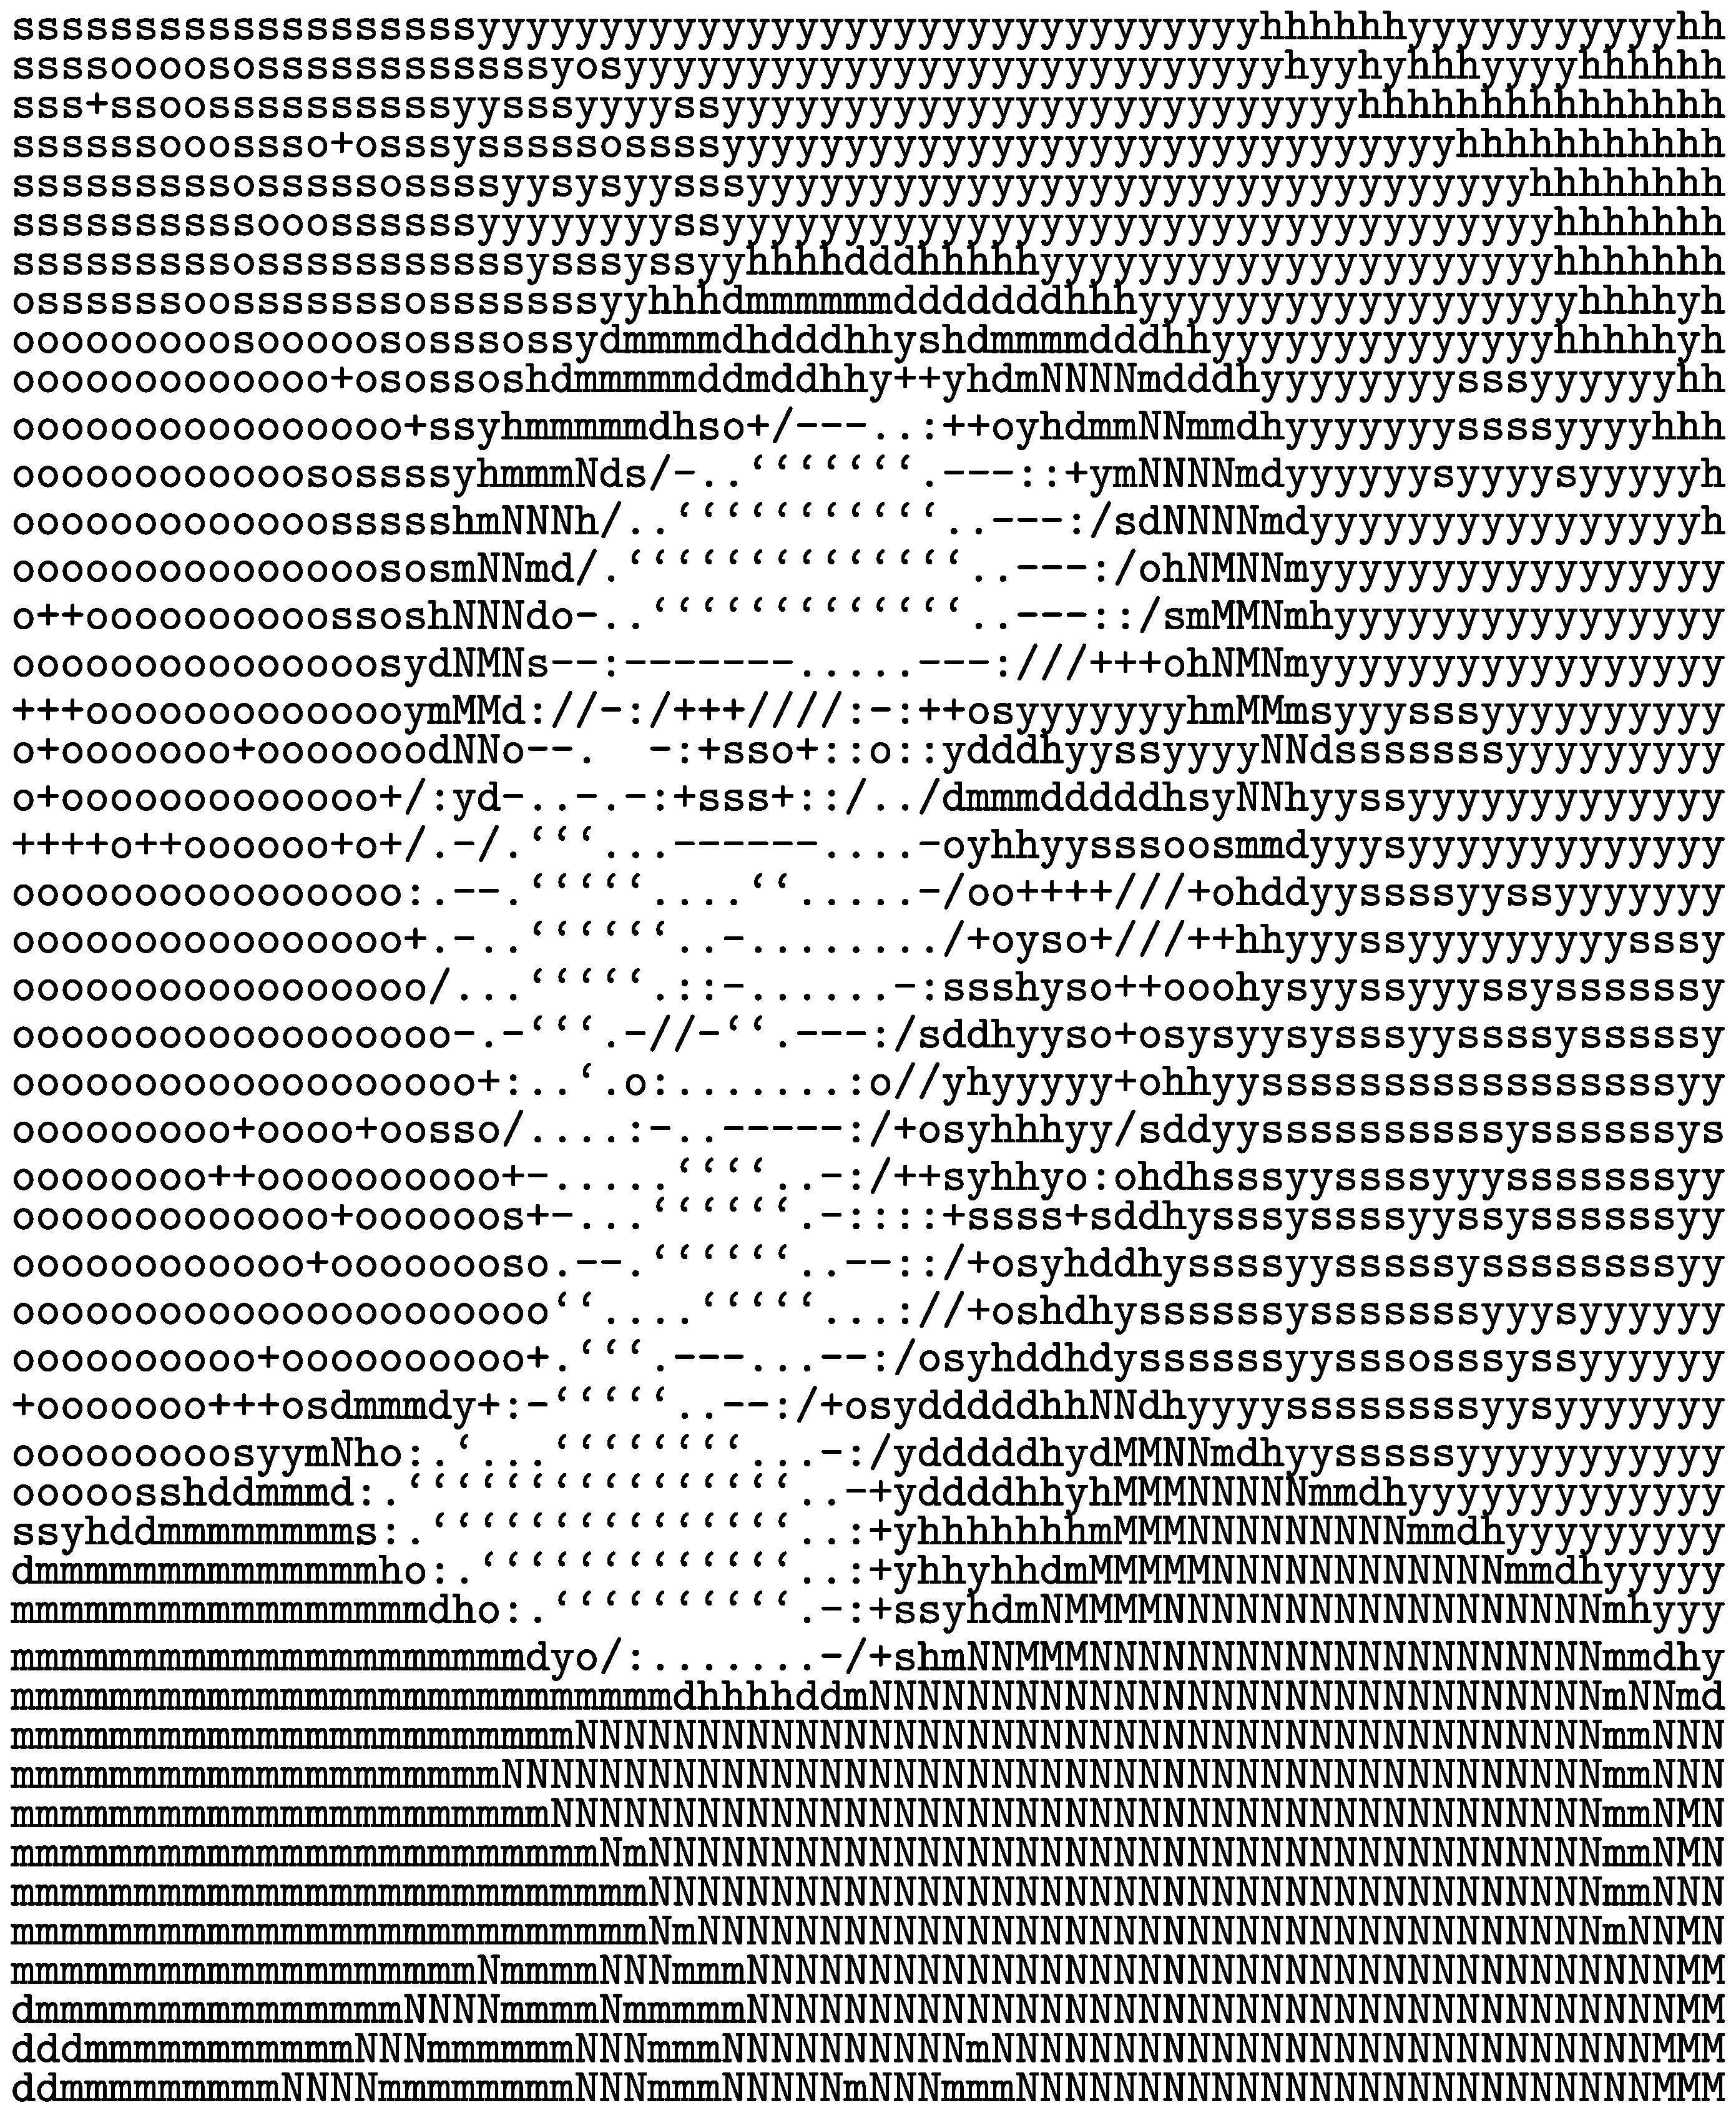
\includegraphics[width=\textwidth /2]{latex-image-1.eps}
\end{center}

\tableofcontents
\include{index}
\include{titlepg}

\mainmatter

\chapter{The Basics}

\begin{center}
\textbf{\begin{huge} September 4, 2011\end{huge}}
\end{center}

\section{Hydrostatic Equilibrium and the Virial Theorem}

\begin{align}
\int \frac{dP}{dr} &= -\rho g\\
&= -\int \frac{\rho GM_r}{r^2}\\
&= -\int \frac{\rho GM}{r^2}4 \pi r^3dr
\end{align}

Let's first solve each side individually and combine the results:

RHS:

\begin{align}
-\int_0^R \frac{GM_r}{r} 4 \pi r^2 \rho dr\\
\frac{dM_r}{dr}=4\pi r^2\rho\\
dM_r = 4 \pi r^2\rho dr\\
-\int_0^R \frac{GM_r}{r} dM_r \equiv U
\end{align}

LHS:

\begin{align}
&=\int_0^R \frac{dP}{dr}4\pi r^3 dr\\
\frac{d}{dr}(P 4 \pi r^3) = \frac{dP}{dr}4\pi r^3 + 3P4\pi r^2\\
&=\int_0^Rdr \lp \frac{d}{dr}\lp P4\pi r^3 \rp - 3P 4\pi r^2 \rp\\
&=\int_0^R \underbrace{dr \cdot  \frac{d}{dr}\lp P4\pi r^3 \rp}_{P 4 \pi r^3 \Bigl\lvert_0^R} - \underbrace{3 \int_0^R 4 \pi r^2drP }_{-3\int dVP}\\
&=P 4 \pi R^3 - P 4 \pi 0^3 - 3\int dVP~,\text{ but $P=0$ at surface, so $P4\pi R^3=0$}
\end{align}

\begin{align}
<P> &= \int_{P(r=0)}^{P(r=R)}dP\\
&= \frac{1}{V}dVP\\
&= \frac{3}{4 \pi R^3}\int dVP
\end{align}

Combining the LHS and RHS, 

\begin{align}
\Aboxed{-3<P>V &= U}
\end{align}

This is the most general version of the Virial Theorem for stars. Now that we have this, let's derive relations between $P$ and $E$. First, what are the properties of stars?

\begin{list}{$\circ$}{}
\item $n=$ \# per unit time
\item $\bar{V}=$ velocity
\item $\bar{p} =$ momentum
\end{list}

Force on a wall $= \frac{\Delta p}{\Delta t}$. $PA = \frac{\Delta p}{\Delta t}$, $P = \frac{\Delta p}{\Delta t}\frac{1}{A}$.\\

\begin{align}
\frac{\Delta p}{\Delta t} = \# \text{ of collisions per unit time $\times~ \Delta p$ per collision}
\end{align}

For particles moving either way, 

\begin{align}
\frac{\Delta p}{\Delta t} &= n\cdot v_x \cdot A \cdot \half\\
\frac{\Delta p_x}{\Delta t} &= nv_xp_xA = PA\\
\frac{\Delta p_y}{\Delta t} &= nv_yp_yA = PA\\
\frac{\Delta p_z}{\Delta t} &= nv_zp_zA = PA\\
\frac{\Delta p}{\Delta t} &=\frac{1}{3}nA\bar{v}\bar{p} = PA\\
\frac{\Delta p}{\Delta t} &=\frac{1}{3}nvp = P\\
\Aboxed{P &= \frac{1}{3}n<pv>}
\end{align}

\subsection{NR Virial Theorem}

For a NR gas of partiles, $p=mv$

\begin{align}
P &= \frac{1}{3}n<mv^2>\\
P &= \frac{2}{3}n<\half mv^2>\\
P &= \frac{2}{3}n<K>~,\text{ KE is the energy per unit particle}\\
P &= \frac{2}{3}K~,\text{ per unit volume}
\end{align}

\begin{align}
U &= -3<P>V\\
&= -3 \left< \frac{2}{3}K\right> V\\
\Aboxed{U &= -2<K>}\\
E_{TOT} &= U + K = \frac{U}{2}
\end{align}

What about a star where the kinetic energy is mostly dominated by relativistic particles?
\subsection{R Virial Theorem}

\begin{align}
P &= \frac{1}{3}n<pc>\\
P &= \frac{1}{3}n\frac{K}{v}\\
U &= 3 \lp \frac{1}{3}nK \rp\\
\Aboxed{U &= -K}\\
E_{TOT} &= U + K = 0
\end{align}

If $E_{TOT} < 0$, the star is bound and stable. If $E_{TOT} = 0$, then the star is unstable. 

\section{Behavior of NR Stars}

For a NR star, $E_{TOT} = -K = \frac{U}{2}$. Let's say the star is losing heat to radiation and thus $E_{TOT}$ is decreasing. Because it's a gravitationally bound system, a loss in $E$ means that the star will contract and heat up. In other words, the star has negative heat capacity. \\

How long will it take for a star to go from $r=R$ to $r=\frac{R}{2}$? 

\begin{align}
\Delta U &\sim \frac{GM^2}{R}\\
&\sim \frac{GM^2}{ \lp\frac{R}{2} \rp}\\
&\sim \frac{2GM^2}{R}
\end{align}

Since we're dealing with Kelvin Helmholtz contraction, let's define a new time scale $t_{KH}$ defined to be $t_{KH} \approx \frac{E}{L}$. For our sun, $t_{KH} \approx 3 \times 10^7$ years $\ll 4.5 \times 10^9$ years, where the latter is the approximate current age of our sun. Therefore, KH contraction cannot explain fully the behavior of the sun; something else must be needed (fusion). 

%%%%%%%%%%%%%%%%%%%%%%%%%%%%%%%%%%%%%%%%%%%%%%%%%%
%%%%%%%%%%%%%%%%%%%%%%%%%%%%%%%%%%%%%%%%%%%%%%%%%%
%%%%%%%%%%%%%%%%%%%%%%%%%%%%%%%%%%%%%%%%%%%%%%%%%%
%%%%%%%%%%%%%%%%%%%%%%%%%%%%%%%%%%%%%%%%%%%%%%%%%%
%%%%%%%%%%%%%%%%%%%%%%%%%%%%%%%%%%%%%%%%%%%%%%%%%%
%%%%%%%%%%%%%%%%%%%%%%%%%%%%%%%%%%%%%%%%%%%%%%%%%%
%%%%%%%%%%%%%%%%%%%%%%%%%%%%%%%%%%%%%%%%%%%%%%%%%%

\chapter{Energy Transport}

\begin{center}
\textbf{\begin{huge} September 6, 2011\end{huge}}
\end{center}

\section{Energy Transport by Conduction}
\begin{figure}[!ht]
\centering
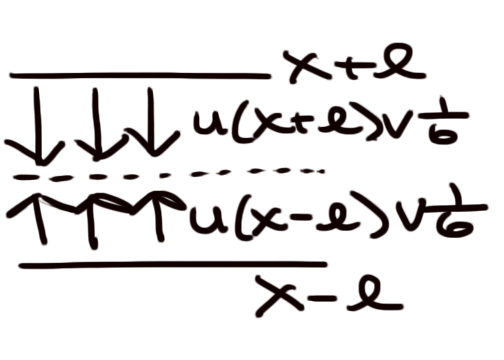
\includegraphics[width=\textwidth /2]{Individual Days/9-6/fig1.png}
\label{fig:1}
\end{figure}

Figure \ref{fig:1} shows the stratification levels of the inside of a star at a given height $x$ with a length $l$  either up or down. \\
\begin{list}{}{}
\item $T$ = temp
\item $u$ = thermal Energy Density
\item $v$ = velocity
\item $l $= mean free path
\end{list}

The factor of $\frac{1}{6}$ is used because we multiply $\frac{1}{3}$ (from 3 degrees of translational freedom) with $\frac{1}{2}$ (from going up and down).

\begin{align}
F \equiv ~\text{net flux of energy} = \frac{1}{6}u(x-l)v - \frac{1}{6}u(x+l)v
\end{align}
Taylor expanding $u(x-l) = u(x) - \frac{du}{dx}l$, we get:

\begin{align}
F = -\frac{1}{3}vl\frac{du}{dx}~,~\text{or more generally,}~F=-\chi \nabla u
\end{align}

\subsection{Mean Free Path}
$\sigma$ is the collisional cross section of an individual particle. Flux can be defined as both $\frac{\text{\#}}{\text{area $\cdot$ time}}$ and $\frac{\text{\# of collisions}}{\text{sec}}$. The probability of colliding is $n \cdot dx \sigma$. The mean free path is the $dx$ where the probability of colliding is 1. $l = \frac{1}{n \sigma}$.\\
For neutral particles, $ R \sim a_0 \sim 0.5$\AA. $\sigma = \pi a_0^2 \sim 10^{-15}$ cm$^2$. In air, $l = \frac{1}{n \sigma}$ where $ n \sim 10^{20}$ cm$^{-3}$ which results in $l = 10^{-5}$ cm. \\

For a gas of charged particles,

\begin{align}
U &= n\frac{3}{2}kT\\
F &= -\frac{1}{3}vl \frac{dU}{dT}\frac{dT}{dx}~,~\text{where}~\frac{dU}{dT}~\text{is the specific heat}\\
\Aboxed{F &= -\frac{1}{2}nklv \frac{dT}{dx}}~.
\end{align}

In the case of a charged particle moving past another charged particle, there is a characterized distance $b$ where the change in trajectory is significant. 

\begin{align}
\frac{q^2}{b} &\sim kT\\
b &\sim \frac{q^2}{kT}\\
\text{effective area }=\sigma &= \pi b^2\\
\Aboxed{\sigma &= \frac{\pi q^4}{(kT)^2}}
\end{align}

\begin{align}
F &=-\frac{1}{2}nklv\frac{dT}{dx}~,v \sim v_{thm} = \sqrt{\frac{kT}{m}}\\
&\sim -\frac{1}{2} \frac{kv}{\sigma}\frac{dT}{dx}\\
&=-\chi \frac{dT}{dx}~,\text{where }\chi =\frac{1}{2}\frac{kv}{\sigma} \pt \frac{T^{5/2}}{\sqrt{m}}
\end{align}

Electrons move faster than protons so they transfer energy much more effectively. Electrons and protons have the same $\sigma$, but the difference in velocities is huge.

\subsection{How important is this energy transport in the sun?}

\begin{align}
F &= -\chi \frac{dT}{dx}\\
L &= 4 \pi R^2 F\\
&\sim 4 \pi R^2 \chi \frac{T_c}{R}~\text{(We're doing a poor man's derivative where $\frac{dT}{dx} = \frac{T_c}{R}$)}\\
L &\sim \frac{k^{7/2} T_c^{7/2} R}{q^4 \ln (\Lambda) \sqrt{m_e}}\\
&\sim 10^{-4} L_\odot \lp \frac{R}{R_\odot} \rp \lp \frac{T_c}{10^7\text{ K} } \rp^{7/2}
\end{align}

Doing this, we get that $L_{conduction} \ll L_\odot$ and therefore electron conduction is unimportant to energy transport. 

\section{Radiation Transport of Energy}
\begin{list}{}{}
\item $U = aT^4$
\item $l = \frac{1}{n \sigma} = \frac{1}{\kappa \sigma}$
\item $\sigma$ = cross section for photons to interact with matter, not with other photons
\end{list}

\begin{align}
F &=-\frac{1}{3}cl \frac{d}{dr}aT^4~,\chi = \frac{4}{3}claT^3 = \frac{4}{3}\frac{caT^3}{n\sigma} \\
&= -\frac{4}{3}claT^3 \frac{dT}{dr}\\
\Aboxed{&=-\frac{4}{3}\frac{caT^3}{\kappa \rho} \frac{dT}{dr}}
\end{align}

For an Ionized plasma with dominant photon-matter interactions through electron scattering (Thomson Scattering),

\begin{align}
m_e \bar{a} &= -e(\bar{E} + \frac{\bar{v}}{c} \times \bar{B})\\
|E| &= |B|\\
m_e\bar{a} &= -e\bar{E}\text{ since $ \frac{\bar{v}}{c} \times \bar{B}$ is small}\\
\bar{a} &= -\frac{e \bar{E}}{m_e}
\end{align}

\begin{align}
P &= \frac{2}{3}\frac{e^4}{c^3 m_e^2}|\bar{E}|^2\\
\sigma F &= P\\
\sigma \frac{c}{4\pi}|\bar{E}| &= \frac{2}{3}\frac{e^4}{c^3 m_e^2}|\bar{E}|^2\\
\Aboxed{\sigma_T &= \frac{8\pi}{3}\frac{e^4}{m_e^2 c^4} = \text{ Thomson cross-section or $e^-$-scattering cross-section}}
\end{align}

\begin{align}
\sigma_T &= \frac{8\pi}{3}r_c^2,~\text{ where $r_c$ is the classical radius of the $e^-$}\\
r_c &=\frac{e^2}{m_e c^2} \approx 2.8 \times 10^{-13} \text{ cm},
\end{align}
which should strike as odd since $e^-$ has no observed structure but still has an "effective radius".

%%%%%%%%%%%%%%%%%%%%%%%%%%%%%%%%%%%%%%%%%%%%%%%%%%
%%%%%%%%%%%%%%%%%%%%%%%%%%%%%%%%%%%%%%%%%%%%%%%%%%
%%%%%%%%%%%%%%%%%%%%%%%%%%%%%%%%%%%%%%%%%%%%%%%%%%
%%%%%%%%%%%%%%%%%%%%%%%%%%%%%%%%%%%%%%%%%%%%%%%%%%
%%%%%%%%%%%%%%%%%%%%%%%%%%%%%%%%%%%%%%%%%%%%%%%%%%
%%%%%%%%%%%%%%%%%%%%%%%%%%%%%%%%%%%%%%%%%%%%%%%%%%
%%%%%%%%%%%%%%%%%%%%%%%%%%%%%%%%%%%%%%%%%%%%%%%%%%

\chapter{Conduction}

\begin{center}
\textbf{\begin{huge} September 8, 2011\end{huge}}
\end{center}

\section{Picking Up Where We Left Off}
\begin{align}
F &= -\frac{4}{3}\frac{caT^3}{\kappa \rho} \frac{dT}{dr} \leftarrow \text{ for radiative diffusion}\\
&= -\frac{1}{3}lc \frac{dU}{dr}
\end{align}

Applying it:

\begin{align}
\frac{dT}{dr} \sim -\frac{T}{R}\\
L \sim \chi M^3~, kT \sim \frac{GM \mu m_p}{R}\\
\chi = \frac{a (\mu m_p)^4 cG^4 \mu_e m_p}{\sigma_T \kappa^4}\\
L \sim 10^{35} \lp \frac{M}{M_\odot} \rp ^3 \text{ ergs/s}\\
L \sim L_\odot~,e^- \text{ conduction $L \ll L_\odot$ so photons are dominating}
\end{align}

$L$ is strictly \textit{NOT} dependent on fusion, it is more dependent on $\frac{dU}{dT}$ of the photons. Fusion creates $E$ and the photons but doesn't determine the rate of energy leaving.\\
$\chi$ is constant, but dependent on the composition of the star. 

\begin{align}
L \pt \mu^4 \mu_e M^3\\
H \rightarrow HE\\
\mu \rightarrow \mu \uparrow\\
L \rightarrow L \uparrow
\end{align}

$L$ was lower in the past. $L$ when the Earth forced was only 20\% of the current $L_\odot$. This brings about the problem that the Earth was supposedly a ball of ice during it's evolution. \\

\begin{align}
\frac{3}{2}nkT > aT^4\\
F &= -\frac{1}{3}lv \frac{dU}{dx}\\
&= -\chi \frac{dT}{dx},\chi = \frac{1}{3}lv \frac{dU}{dT}\\
\frac{F_{rad}}{F_{e^-}} &= \frac{-\chi_{rad}}{-\chi_{e^-}}, \frac{dT}{dx}\text{ is the same for both}\\
&\sim \frac{l_\gamma}{l_{e^-} }\frac{ c}{v_{e^-} }\frac{aT^4}{\frac{3}{2}nkT}
\end{align}

$ \frac{l_\gamma}{l_{e^-} } \ggg 1$, $\frac{ c}{v_{e^-}} \gg 1$, and $\frac{aT^4}{\frac{3}{2}nkT} \ll 1$.\\

\begin{align}
F = -\frac{4}{3}\frac{caT^4}{n \sigma} \frac{dT}{dr}
\end{align}

We want to find the time for thermal energy to leak out by photon diffusion.

\begin{align}
t_{KH} &= \frac{E}{L}\\
L &\sim 4 \pi R^2 \frac{4}{3}aT^3 \frac{1}{n\sigma}\frac{T}{R}\\
&= \frac{\frac{3}{2}nkT \cdot \dfrac{4}{3}\pi R^3}{ \lp \dfrac{4 \cdot 16 \pi aT^4R}{R3n\sigma} \rp}\\
&=\frac{\frac{3}{2}nkTR^2n\sigma}{4aT^4c}\\
&\sim \frac{nkT}{aT^4}\frac{R^2}{lc}\\
&\sim \frac{nkT}{aT^4}t_{RW}~,\text{ where $t_{RW}=\frac{R^2}{lc}=$ random walk time}
\end{align}

\begin{align}
<|D|^2>&=Nl^2~,\text{ where $N = $ number of steps}\\
<|D|^2>^{1/2} &= \text{ RMS Distance = typical distance a photon will find itself after $N$ scatterings}\\
&= \sqrt{N}l
\end{align}

What is $N$ so that the photon leaves the star?

\begin{align}
<|D|^2>^{1/2} &=R\\
N &\sim \lp \frac{R}{l} \rp^2\\
\frac{R}{l} \sim 10^{11},N\sim 10^{22}
\end{align}

How long does it take to get out? 

\begin{align}
Nt_{step} = t_{esc} = N\frac{l}{c} \sim \lp \frac{R}{l} \rp^2 \cdot \frac{l}{c} \sim \frac{R^2}{lc}\\
\sim 10^4 \text{ years for our sun}
\end{align}

If photons didn't bounce around, it would escape in 2 seconds. ($\nu_e$ can get out in about 2 seconds, $l_\nu$ must be greater than $R_\odot$) Also, the time it takes for heat to diffuse throughout a room is: $\frac{R^2}{lv_{thm}}$.

\begin{align}
F &= -\frac{4}{3}\frac{caT^4}{n \sigma} \frac{dT}{dr}\\
&= -lc \frac{d}{dr}\frac{1}{3}aT^4\\
F_r &= -lc\frac{d}{dr}P_{rad}~,\text{ we must be careful, $F$ and $L$ depend on $r$}\\
\frac{L_r}{4\pi r^2} &= -lc \frac{d}{dr}P_{rad}\\
-\frac{L_r}{4\pi lc r^2} &= \frac{d}{dr}P_{rad}\\
-\frac{L_r \kappa \rho}{4\pi c r^2} &= \frac{d}{dr}P_{rad}\\
\end{align}

We're interested in how $P_{rad}$ changes with $P_{tot}$. 

\begin{align}
\frac{dP_{rad}}{dP} = \frac{L_r \kappa}{4 \pi G M_r c} \equiv \frac{L_r}{L_{EDD}}
\end{align}

Roughly, if $P_{rad} \sim P_{tot}$, then $L_r \sim L_{EDD}$.

\subsection{Eddington Luminosity}

\begin{list}{}{}
\item $F_g = -\frac{GMm}{r^2}$
\item $F_{rad} = \frac{dp}{dt}$
\item $p_{proton} = \frac{E}{c} = \frac{h \nu}{c} = \frac{h}{\lambda}$
\end{list}

What is the total $p$ per unit time produced by the star? $\sum\limits{_i^\infty} p_i $ is too hard...

\begin{align}
p_{photon} = \frac{E}{c} = \frac{L}{c}\\
F_{Rad} = \frac{dp}{dt} = \frac{L}{c 4\pi r^2} \sigma
\end{align}

The Eddington Luminosity is where the radiation force equals the forge of gravity. The Eddington "Limit" is:

\begin{align}
L_{EDD} = \frac{4 \pi G Mc}{\sigma /m} = \frac{4 \pi G Mc}{\kappa}
\end{align}

If $L > L_{EDD}$, $F_{rad} > F_{grav}$, and material is "blown" out. 

\subsection{Fully Ionized H}

\begin{list}{$\circ$}{}
\item $L_{EDD} = \frac{4 \pi GMc}{\kappa}$
\item $\kappa = \frac{\sigma_T}{m}$
\item $l = \frac{1}{n \sigma} = \frac{1}{n_e \sigma_T} = \frac{1}{\kappa \sigma}$
\item For fully ionized $H$, $\mu_e =1$
\item since photons are only interacting with $e^-$ and not $p$, $\mu = 1 = \mu_e$
\end{list}

\begin{align}
\kappa &= \frac{\sigma_T}{m}\\
&= 0.4\text{ cm}^2\text{ g}^{-1}
\end{align}

\begin{align}
L_{EDD} = 1.3 \times 10^{38} \lp \frac{M}{M_\odot} \rp \text{ ergs s}^{-1}
\end{align}

\begin{list}{}{}
\item If $L \sim L_{EDD}$, $F_{rad} \sim F_{grav}$ which results in the radiation force not being important in the sun. It's dominated by gas pressure.
\item As $M \uparrow, L_{EDD} \uparrow$ so higher $M$ means $P_{rad}$ becomes more important $\rightarrow$ it becomes the dominant force
\end{list}

%%%%%%%%%%%%%%%%%%%%%%%%%%%%%%%%%%%%%%%%%%%%%%%%%%
%%%%%%%%%%%%%%%%%%%%%%%%%%%%%%%%%%%%%%%%%%%%%%%%%%
%%%%%%%%%%%%%%%%%%%%%%%%%%%%%%%%%%%%%%%%%%%%%%%%%%
%%%%%%%%%%%%%%%%%%%%%%%%%%%%%%%%%%%%%%%%%%%%%%%%%%
%%%%%%%%%%%%%%%%%%%%%%%%%%%%%%%%%%%%%%%%%%%%%%%%%%
%%%%%%%%%%%%%%%%%%%%%%%%%%%%%%%%%%%%%%%%%%%%%%%%%%
%%%%%%%%%%%%%%%%%%%%%%%%%%%%%%%%%%%%%%%%%%%%%%%%%%

\chapter{Convection}

\begin{center}
\textbf{\begin{huge} September 13, 2011\end{huge}}
\end{center}

\section{Convection}
Second Law of Thermodynamics: $TdS = dE + PdV$, which isn't all that useful for stars, really.
\begin{list}{}{}
\item $U = \frac{E}{\mu}$: Energy per unit mass
\item $s = \frac{S}{U}$: Entropy per unit mass
\item $M =$ conserved, $l$ is small
\item $\rho = \frac{M}{V}, V = \frac{M}{\rho} \rightarrow \boxed{dV = -d\rho \frac{M}{\rho^2}}$
\item $\frac{TdS = dE + PdV}{\mu} = \boxed{ TdS = dU - \frac{P}{\rho^2}d\rho }$  : second law, for astrophysicists
\end{list}

\subsection{Review of the Adiabatic Process}

\begin{align}
\epsilon = E/\text{unit volume},\text{ NR}: P &= \frac{2}{3} \epsilon\\
\text{R}: P &= \frac{1}{3} \epsilon\\
U = \frac{\epsilon}{\rho} = \frac{P}{\rho} = \phi U~,\text{ where $\phi$ is either $1/3$ or $2/3$}\\
dU = \frac{P}{\rho^2}d\rho = \phi U\frac{d\rho}{\rho}\\
\frac{dU}{U} = \phi \frac{d\rho}{\rho}\\
U \pt \rho^\phi~,\text{ for an adiabatic process}\\
P \pt \rho U \pt \rho ^{\phi+1} \pt \rho^{\gamma}~,  \phi + 1  = \gamma =\text{ the adiabatic index}\\
\end{align}

\begin{align}
\text{For a NR gas: } \phi = \frac{2}{3}, \gamma = \frac{5}{3}~,P\pt \rho^{5/3}, T \pt \rho^{2/3}\text{ for an adiabatic process}\\
\text{For a R gas: } \phi = \frac{1}{3}, \gamma = \frac{4}{3}~,P\pt \rho^{4/3}, T \pt \rho^{1/3}\text{ for an adiabatic process}
\end{align}

\subsection{What is the Entropy of an Ideal Gas?}

\begin{align}
TdS &= dU - \frac{P}{\rho^2}d\rho\\
\frac{TdS}{U} &= \frac{dU}{U} - (\gamma - 1)\frac{U\frac{d\rho}{\rho}}{U}\\
U &=\frac{P}{\rho}\frac{1}{\gamma -1} = \frac{1}{\gamma - 1} \frac{kT}{m}\\
\frac{m(\gamma -1)}{k}dS &= \frac{dU}{U} - (\gamma -1)\frac{d\rho}{\rho}\\
\frac{m(\gamma - 1)}{k}s &= \ln U - (\gamma - 1)\ln \rho + c\\
\Aboxed{s &= \frac{k}{m}\frac{1}{\gamma - 1} \ln \lp \frac{U}{\rho^{\gamma - 1}} \rp  +c}\\	
s &= \frac{k}{m} \frac{1}{\gamma -1} \ln \lp \frac{P}{\rho^\gamma} \rp + c
\end{align}

For an adiabatic process, $s=0 \rightarrow \frac{k}{m} \frac{1}{\gamma -1} \underbrace{\ln \lp \frac{P}{\rho^\gamma} \rp}_{P \pt \rho^\gamma} + c$

\begin{align}
\frac{Tds}{dt} &= \underbrace{\frac{dU}{dt}}_{\text{heating}} - \underbrace{\frac{P}{\rho^2}\frac{d\rho}{dt}}_{\text{cooling}}\\
&= \underbrace{E_{heat}}_{\text{fusion}} - \underbrace{\frac{1}{\rho}(\bar{\nabla} \cdot \bar{F})}_{\text{photon convection}}
\end{align}

Say a blob is gaining/losing heat. $E_{fusion}$ is the heating per mass per time and $\bar{F}$ is the flux of $E$. In general:

\begin{align}
\text{total cooling} &= \int \bar{F}\cdot d\bar{A}\\
&= \int \bar{\nabla} \cdot \bar{F} d\bar{V}\\
\text{cooling per unit $V$} &= \bar{\nabla} \cdot \bar{F}\\
\text{cooling per unit mass} &= \frac{1}{\rho}(\bar{\nabla} \cdot F)
\end{align}

If a blob moves up a distance $dr$, given $T(r), P(r),$ and $\rho(r)$, is the fluid buoyantly stable? i.e. $\rho_{blob} \gtrless \rho_*$? We'll be making 2 assumptions which we will then confirm \textit{post-facto}. 
\begin{list}{$\circ$}{}
\item Motion is adiabatic $\leftarrow$ valid if the time scale to move ($\sim$ 1 month) is sufficiently smaller than the time to exchange heat with the surroundings ($\sim10^7$ years)
\item $P_{blob} = P_*$ at all times; in pressure equilibrium with surroundings
\end{list}

The time scale to establish HE: $\sim\frac{1}{\sqrt{G\rho}} \sim 1 $ hr $\ll$ time to move $dr$, which is about a month. If it's adiabatic, $s_{blob} = s \ne s_*$ in general, where $s_{blob}$ is the blob at the new position, $s$ is the initial entropy, and $s_*$ is the background entropy of the star at the new position.\\

\begin{center}
\begin{tabular}{c|c}
\hline
$\dfrac{ds}{dr} < 0$ & $\dfrac{ds}{dr} > 0$\\ \hline
$s>s_*$ & $s < s_*$\\ \hline
$s_{blob} > s_*$ & $s_{blob}< s_*$\\ \hline
$P_{blob} = P_*$ & $P_{blob} = P_*$\\ \hline
$\rho_{blob} < \rho_*$ & $\rho_{blob} > \rho_*$ \\ \hline
buoyancy unstable, rises & sinks back down (stable)\\
\hline
\end{tabular}
\end{center}

%%%%%%%%%%%%%%%%%%%%%%%%%%%%%%%%%%%%%%%%%%%%%%%%%%
%%%%%%%%%%%%%%%%%%%%%%%%%%%%%%%%%%%%%%%%%%%%%%%%%%
%%%%%%%%%%%%%%%%%%%%%%%%%%%%%%%%%%%%%%%%%%%%%%%%%%
%%%%%%%%%%%%%%%%%%%%%%%%%%%%%%%%%%%%%%%%%%%%%%%%%%
%%%%%%%%%%%%%%%%%%%%%%%%%%%%%%%%%%%%%%%%%%%%%%%%%%
%%%%%%%%%%%%%%%%%%%%%%%%%%%%%%%%%%%%%%%%%%%%%%%%%%
%%%%%%%%%%%%%%%%%%%%%%%%%%%%%%%%%%%%%%%%%%%%%%%%%%

\chapter{More Convection}

\begin{center}
\textbf{\begin{huge} September 15, 2011\end{huge}}
\end{center}

\section{Models}
Blob's motion is adiabatic: $s_{blob} = s \ne s_*$. The blob is in pressure and pressure equilibrium with it's surroundings. The time scale for the blob to move is $\ll t_{{\text dynamic}}$ or $t_{{\text sound~crossing}}$. 

\begin{align}
s \pt \ln \lp \frac{P}{\rho^\gamma} \rp : \frac{ds}{dr}<0~, s_{blob} = s > s_*~,\rho_{blob} < \rho_*
\end{align}

At the new position, $a = g \frac{\Delta \rho}{ \rho} = |\bar{g} | \lp \frac{\rho_* - \rho_{blob}}{\rho_{blob}} \rp$. If $\rho_{blob} > \rho_*$, $a$ is negative and it goes back down. If $\rho_{blob} < \rho_*$, then $a$ is positive.

\subsection{Background Stellar Model}

\begin{align}
\boxed{\rho_* = \rho + \frac{d \rho}{dr} \delta r}~,\text{ where $ \frac{d \rho}{dr}$ is the $\rho$ gradient of the stellar model}
\end{align}

This, however, is quite boring. 

\begin{align}
P_* &= \rho + \frac{d\rho}{dr}\delta r\\
&= P_{blob} = P  + \delta P\\
\delta P &= \frac{dP}{dr}\delta r
\end{align}

\subsection{Blob Model}

\begin{align}
\rho_{blob} &= \rho + \underbrace{\lp \frac{\delta \rho}{\delta P} \rp_s}_{\text{adiabatic}} \delta P~, \text{ able to calculate $\delta P$ from $P_{\text{blob}} = P_*$}\\
P &\pt \rho^\gamma\\
\lp \frac{\delta P}{\delta \rho} \rp_s &= \gamma \frac{P}{\rho}\\
\lp \frac{\delta \rho}{\delta P}\rp_s = \frac{\rho}{\gamma P}\\
\rho_{blob} &= \rho + \frac{\rho}{\gamma}\frac{\delta P}{P}\\
\Aboxed{\rho_{blob} &= \rho + \frac{\rho}{\gamma} \frac{d \ln P}{dr} \delta r}
\end{align}

\begin{align}
a &= g  \lp \frac{\rho_* - \rho_{blob}}{\rho_{blob}} \rp\\
&= g \lp \frac{\rho + \frac{d\rho}{dr} \delta r}{\rho + \frac{\rho}{\gamma} \frac{d \ln P}{dr}\delta r} - 1 \rp~,\text{ assuming that $\delta r$ is really small}
\end{align}

\begin{align}
a &\equiv -N^2\delta r\\
N &= -g \lp \frac{d \ln \rho}{dr} - \frac{1}{\gamma} \frac{d \ln P}{dr} \rp\\
&= \frac{\gamma -1}{\gamma} \frac{m}{k}g \frac{ds}{dr}
\end{align}

$[N] = \frac{1}{s}$, the Brunt-V\"ais\"al\"a Frequency. Whether or not convection sets in or not is only dependent on $\frac{ds}{dr}$. 

\begin{align}
a = \frac{d^2}{dt^2}\delta r = -N^2 \delta r\\
\boxed{\frac{d^2}{dt^2}\delta r + N^2 \delta r = 0}~,\text{ Equation of Motion}
\end{align}

If $N^2 > 0$, then $\delta r \pt e^{iNt} \pt  \cos(Nt)  + i\sin(Nt)$. This is a stable oscillatory solution. If you push it a little bit, it'll oscillate. If $N^2 < 0, \frac{ds}{dr} < 0, \delta r \pt e^{|N|t}$, which is an exponentially growing solution on a time scale $\frac{1}{N}$ and is dubbed "convection". Say for example we know $dP, d\rho, ds$, then we know if it's spontaneously boiling.\\

\subsection{Will Convection Set In?}

Convection sets in if:

\begin{align}
\frac{ds}{dr} < 0\\
N^2 < 0\\
s &\pt \ln \lp \frac{P}{\rho^\gamma} \rp\\
 &\pt \ln \lp \frac{T^\gamma}{P^{\gamma -1}} \rp\\
P = \frac{\rho kT}{\mu m_p}\\
\rho \pt \frac{P}{T}~.
\end{align}

\begin{align}
\gamma \frac{d \ln T}{dr} &< ( \gamma - 1) \frac{d \ln P}{dr}\\
\underbrace{\frac{d \ln T}{dr}}_{\text{$-$ sign}} &< \frac{\gamma -1}{\gamma}\underbrace{\frac{d \ln P}{dr}}_{\text{$-$ sign}}\\
\Aboxed{\Bigl\lvert \frac{d \ln T}{dr} \Bigl\lvert &> \frac{\gamma -1}{\gamma} \Bigl\lvert \frac{d \ln P}{dr} \Bigl\lvert} \\
\text{or}\\
\Bigl\lvert \frac{d \ln T}{d \ln P	} \Bigl\lvert &> \frac{\gamma - 1}{\gamma} = \frac{2}{5}~,\gamma = \frac{5}{3}
\end{align}

We can calculate $\frac{dT}{dr}$ if the photons carry the energy.

\begin{align}
\Bigl\lvert \frac{d \ln T}{dr} \Bigl\lvert &> \frac{\gamma -1}{\gamma} \Bigl\lvert \frac{d \ln P}{dr} \Bigl\lvert\\
\text{Combine HE \& RD: } \frac{dP_{rad}}{dP} &= \frac{L_r \kappa}{4 \pi GM_r c}\\
\frac{P}{P_{rad}}\frac{dP_{rad}}{dP} &= \frac{L_r \kappa}{4 \pi GM_r c}\frac{P}{P_{rad}}~,\frac{P}{dP} = \frac{1}{d \ln P}\\
\Aboxed{\frac{d \ln P_{rad}}{d \ln P} &=4 \frac{d \ln T}{d \ln P}}
\end{align}

Quick note about the $d \ln T$ stuff: take for example $P\pt T_{rad}^4$. $\ln P_{rad} \pt 4 \ln T +$ constant. $\frac{d}{d \ln T} \ln P_{rad} = \frac{d}{d \ln T}4 \ln T +$ constant$= 4$.\\
If photons carry the energy, can directly calculate: 

\begin{align}
\boxed{\frac{d \ln T}{d \ln P} = \frac{1}{4} \frac{P}{P_{rad}} \frac{L_r \kappa}{4 \pi GM_rc}}
\end{align}

Another way to think about it is that if 

\begin{align}
\frac{d \ln T}{d \ln P} > \frac{\gamma -1}{\gamma}~,
\end{align}

then convection sets in.

\section{Our $\odot$}

For our sun, convection occurs in a radius about $r \gtrsim 0.7 R_\odot$. At the enter of the sun, $T\sim 10^7$ K. At larger $r$, $T \downarrow$ and $\kappa \uparrow$. 

\begin{align}
\frac{d \ln T}{d \ln P} > \frac{2}{5}~,\text{ at higher $r$, convection is determined by $\kappa$}
\end{align}

In the region between $0 < r \lesssim 0.7R_\odot$, the sun is relatively much hotter than its other parts and thus photons can carry the energy out. The $l$ per photons is relatively large and streaming out isn't a problem. As you extend outwards, however, $T \downarrow, \kappa \uparrow$, resulting in a higher $N$ (where in this case $N$ is the number of RW steps). Photons now have trouble moving the energy and convection takes over. \\

$M < M_\odot, T < T_\odot, \kappa \uparrow$, and more convection. For stars with $M \lesssim \frac{1}{3}M_\odot$, they are fully convective. $M > M_\odot, T > T_\odot, \kappa \downarrow$, the surface convection zone goes away, BUT the core now becomes convective. What actually happens when convection moves energy?

\section{Energy Transport by Convection}

Let's say there are two blobs, one with a high $\rho$ and low $T$ and another with a low $\rho$ and a high $T$. The blobs with lhgh $\rho$ will sink and the blob with low $\rho$ will rise. This makes sense, hot stuff rises, cold stuff sinks. 

\begin{align}
v_c = \text{ typical convective velocity}\\
F_c &\sim \frac{1}{2}\rho v_c^2 \cdot v_c \\
\Aboxed{&\sim \frac{1}{2} \rho v_c^3}\\
\text{OR}\\
\Aboxed{F_c &\sim \rho \Delta E \cdot v_c}
\end{align}

Since $d\rho$ is so small, able to use either. Let's determine the $v_c$ through the work done by buoyancy. When a blob rises from one position to another, it moves from a region of high $P$ to a region of lower $P$. The blob shares energy with it's surroundings and must enlarge to conserve mass. 

\begin{align}
l \equiv \alpha H~,\text{ H is the scale height},H = \lp \frac{d \ln P}{dr} \rp^{-1}
\end{align}

How much energy goes the blob gain?

\begin{align}
a \equiv |N|^2\delta r\\
E_{gained/mass} = \frac{1}{2}\rho v_c^2\\
v_c^2 &= |N|^2 \delta r\\
v_c^2 &= |N|^2l^2\\
&= \alpha^2 H^2 |N|^2~,|N|^2 = g\frac{1}{c_p} \frac{ds}{dr}
\end{align}

%%%%%%%%%%%%%%%%%%%%%%%%%%%%%%%%%%%%%%%%%%%%%%%%%%
%%%%%%%%%%%%%%%%%%%%%%%%%%%%%%%%%%%%%%%%%%%%%%%%%%
%%%%%%%%%%%%%%%%%%%%%%%%%%%%%%%%%%%%%%%%%%%%%%%%%%
%%%%%%%%%%%%%%%%%%%%%%%%%%%%%%%%%%%%%%%%%%%%%%%%%%
%%%%%%%%%%%%%%%%%%%%%%%%%%%%%%%%%%%%%%%%%%%%%%%%%%
%%%%%%%%%%%%%%%%%%%%%%%%%%%%%%%%%%%%%%%%%%%%%%%%%%
%%%%%%%%%%%%%%%%%%%%%%%%%%%%%%%%%%%%%%%%%%%%%%%%%%

\chapter{Finishing Convection}

\begin{center}
\textbf{\begin{huge} September 20, 2011\end{huge}}
\end{center}

\section{Convection Continued}

\begin{align}
a = |N|^2 \delta r\\
|N|^2 &= \frac{g}{c_p} \Bigl\lvert \frac{ds}{dr} \Bigl\lvert\\
&= \frac{g}{H} \Bigl\lvert \frac{H}{c_p} \frac{ds}{dr} \Bigl\lvert\\
v_c^2 = a \delta r = |N|^2 \delta r^2\\
\delta r \equiv \alpha H\\
v_c = \alpha c_s \Bigl\lvert \frac{H}{c_p} \frac{ds}{dr} \Bigl\lvert^{1/2}\\
F = \frac{1}{2}\rho v_c^3 = \frac{1}{2} \rho \alpha ^3 c_s^3 \Bigl\lvert \frac{H}{c_p} \frac{ds}{dr} \Bigl\lvert ^{3/2}\\
c_s^2 = \frac{kT}{\mu m_p} = \frac{P}{\rho}
\end{align}

We wanted to find the $F_r = -\frac{4}{3} \frac{caT^3}{\kappa \rho}\frac{dT}{dr}$ equivalent for convection. $F = \frac{1}{2}\rho v_c^3 = \frac{1}{2} \rho \alpha ^3 c_s^3 \Bigl\lvert \frac{H}{c_p} \frac{ds}{dr} \Bigl\lvert ^{3/2}$ gives the $v_c$ and $\frac{ds}{dr}$ given the flux. \\

$\Bigl\lvert \frac{H}{c_p} \frac{ds}{dr} \Bigl\lvert \sim 10^{-6}$, $s \sim c_p$, so $\frac{\Delta s }{s} \sim 10^{-6}$ on a length scale $\sim H$. Ergo, $s$ = constant in the convection zone. This replaces $F_r = -\frac{4}{3} \frac{caT^3}{\kappa \rho}\frac{dT}{dr}$. Let's assume $P \pt \rho^\gamma$ \& $\frac{dP}{dr} = -\rho \frac{GM_r}{r^2}$. 

\begin{align}
\frac{dM_r}{dr} = 4 \pi r^2 \rho\\
\frac{d}{dr} \lp \frac{r^2}{\rho} \frac{dP}{dr} = -\rho GM_r \rp\\
\frac{d}{dr} \lp \frac{r^2}{\rho	} \frac{dP}{dr} \rp = -4\pi r^2 G\rho
\end{align}

But... if $P = K \rho^\gamma$, $\frac{dP}{dr} = \gamma K \rho^{\gamma-1} \frac{d\rho}{dr}$! These kinds of models are called:

\subsection{Polytropic Models}

\begin{align}
P &= K\rho^\gamma\\
&= K \rho^{1 + 1/n}, \gamma = 1 + \frac{1}{n}, \text{ where n is the polytropic index}
\end{align}

\begin{align}
\theta = \lp \frac{\rho}{\rho_c} \rp ^{1/n}~,\rho_c = \rho(r=0)\\
\zeta = \frac{r}{a}~, a = \sqrt{\frac{(n+1) K \rho_c ^{\frac{1}{n} -1}}{4 \pi G}}~,[a] = \text{ cm}
\end{align}

\begin{align}
\underbrace{\boxed{\frac{1}{\zeta^2} \cdot \frac{d}{d\zeta} \lp  \zeta^2 \frac{d\theta}{d\zeta} \rp = -\theta^n}}_{\text{Lane-Emden Equation}}
\end{align}

Boundary conditions:

\begin{align}
\theta (0) = 1\\
\frac{d \theta}{d \zeta} \Bigl\lvert_{r=0}\\
\frac{d \theta}{d \zeta} \pt \frac{d \rho}{dr} \pt \frac{dP}{dr} \sim -\frac{\rho GM_r}{r^2} \pt r \text{ as } r \rightarrow 0\\
\frac{dM_r}{dr} = 4 \pi r^2 \rho\\
M_r \sim \rho r^3
\end{align}

Let's look at the properties of a fully convective star of low mass. Low mass $\rightarrow$ low $T$ $\rightarrow$ high $\kappa$. 

\subsection{$M_* < \frac{1}{3} M_\odot$ on Main Sequence - Pre and Post-Stars Too (Giants)}

For stars with photons carrying the energy out, $L \pt M^3$ if $\sigma = \sigma_T$. For fully convective stars, $L = 4 \pi R^2 F_c$, where $F_c = \rho v_c^3 \pt \Bigl\lvert \frac{ds}{dr} \Bigl\lvert^{3/2}$. Let's look at the surface where photons are carrying the energy out. 

\begin{align}
\text{s = constant}\\
P \pt \rho^{5/3} \pt T^{5/2}\\
\rho T \pt \rho^{5/3}, T \pt \rho^{2/3}\\
\frac{P_c}{P_{photons}} = \lp \frac{T_c}{T_{eff}} \rp ^{5/2},\text{ now use V.T. to relate $T_c$ and $M$ \& $R$.}
\end{align}
\begin{center}
{\Huge BUT}
\end{center}
We know that this is a $n=\sfrac{3}{2}$ polytrope so $kT_c = .54 \frac{GM\mu m_p}{R}$

\begin{align}
P_c = 0.77 \frac{GM^2}{R^4}\\
\frac{dP}{dr} = -\rho \frac{GM_r}{r^2}\\
\frac{P_c}{R} \sim \frac{M}{R^3}\frac{GM}{R^2}\\
P_c \sim \frac{GM^2}{R^4}
\end{align}

\begin{align}
\frac{1}{\kappa_{ph}\rho_{ph}} &= \frac{kT_{eff}}{mg} \\
&= \frac{kT_{eff}R^2}{GMm}\\
\frac{\rho_{ph}kT_{eff}}{m} &= \frac{g}{\kappa_{ph}}\\
&\equiv P_{ph}\\
& = \frac{GM}{R^2\kappa_{ph}}
\end{align}

Now all that's left is $\kappa$. $\kappa_{ph}(\rho_{ph},T_{ph})~, \kappa_{ph} \sim 3 \times 10^{-31} \rho_{ph}^{1/2} T_{eff}^9$. Now we have $\frac{\rho_{ph} kT_{eff}}{m} = \frac{g}{\kappa_{ph}}$. In this example, $\kappa = \kappa_{H^-}$ and $T_{eff} \sim 3000 \sim 10^4$ K. Now we can solve:

\begin{align}
\frac{P_c}{P_{ph}}&= \lp \frac{T_c}{T_{eff}} \rp^{5/2}\\
T_{eff} &= T_c \lp \frac{P_{ph}}{P_c	} \rp ^{2/5}\rightarrow T_{eff}(M,R)~,
\end{align}

and from here you can solve for $T_c(M,R), P_c(M,R), P_{ph}(T_{eff},M,R)$.\\

We're going to assume that $s=$ constant and some other stuff about polytropes. $l \sim H \rightarrow P_{ph}(M,R,T_{eff})$ to get:

\begin{align}
\Aboxed{T_{eff} &\approx 3000 \text{ K }\lp \frac{M}{M_\odot} \rp^{1/7} \lp \frac{R}{R_\odot} \rp^{1/49}}\\
\Aboxed{L = 4 \pi R^2 \sigma T_{eff}^4 &\sim 0.1 L_\odot \lp \frac{M}{M_\odot} \rp^{4/7} \lp \frac{R}{R_\odot} \rp^{102/49}}
\end{align}
for a fully convective star; this is analogous to the $L \pt M^3$ for a radiative star
\begin{align}
T_{eff} &\approx 3000 \text{ K } \lp \frac{L}{L_\odot} \rp^{1/102} \lp \frac{R}{R_\odot} \rp^{7/51}
\end{align}

But the dependence on $M$ and $R$ are so low that fully convective stars share the same $T_{eff} \sim 3000-4000$ K and are pretty much located on the Hayashi Line.

%%%%%%%%%%%%%%%%%%%%%%%%%%%%%%%%%%%%%%%%%%%%%%%%%%
%%%%%%%%%%%%%%%%%%%%%%%%%%%%%%%%%%%%%%%%%%%%%%%%%%
%%%%%%%%%%%%%%%%%%%%%%%%%%%%%%%%%%%%%%%%%%%%%%%%%%
%%%%%%%%%%%%%%%%%%%%%%%%%%%%%%%%%%%%%%%%%%%%%%%%%%
%%%%%%%%%%%%%%%%%%%%%%%%%%%%%%%%%%%%%%%%%%%%%%%%%%
%%%%%%%%%%%%%%%%%%%%%%%%%%%%%%%%%%%%%%%%%%%%%%%%%%
%%%%%%%%%%%%%%%%%%%%%%%%%%%%%%%%%%%%%%%%%%%%%%%%%%

\chapter{Star Formation}

\begin{center}
\textbf{\begin{huge} September 22, 2011\end{huge}}
\end{center}

\section{Star Formation}

Gas in galaxies comes in multiple "phases". It's still a gas, just a broad range with particular characteristics. They have different $\rho$ \& $T$ with comparable $P$. Hot, low $\rho$ gas is mostly in the form of hot ISM. Stars form from \textbf{cold molecular clouds}. What are the conditions for a cold molecular gas cloud to collapse? 

\begin{align}
|U| &\geq |K|\\
\frac{GM}{R^2} &\gtrsim \Bigl\lvert \frac{dP}{dr} \Bigl\lvert\\
\text{self gravity of cloud} &\gtrsim \frac{3}{2}NkT\\
&\approx \frac{M}{m_p}kT
\end{align}

If $M \gtrsim \frac{RkT}{Gm_p}$, then it will collapse. 

\begin{align}
\rho &\approx \frac{M}{R^3}\\
R &\sim \lp \frac{M}{\rho} \rp^{1/3}\\
M^{2/3} &\gtrsim \frac{kT}{Gm_p \rho^{1/3}}\\
\Aboxed{M_J &\geq \lp \frac{k}{Gm_p} \rp^{3/2} \frac{T^{3/2}}{\sqrt{\rho}}}~,M_J = {\text{ Jeans Mass}}\\
\frac{GM^2}{R} &\geq \underbrace{\frac{MkT}{m_p}}_{c_s^2} \\
\text{if } \frac{1}{\sqrt{G\rho}} &\leq \frac{R}{c_s}~,\text{ then if $t_{FF} < t_{sound}$, and it will collapse}
\end{align}

Stars are more prone to collapse if they have lower $T$ and higher $\rho$. Stars form from cold molecular clouds because they are the most unstable.

\begin{align}
M_J &\approx 50 M_\odot \frac{\lp \frac{T}{10K}\rp^{3/2}}{\lp \frac{\text{n}}{100} \text{ cm}^{-3} \rp^{1/2}}\\
R_J &= \lp \frac{M_J}{\rho} \rp^{1/3}\\
&\approx 3 \text{ pc} \frac{(\frac{T}{10K})^{1/2}}{(\frac{\text{n}}{100}\text{ cm}^{-3})^{1/2}}
\end{align}

If a star has $M>M_J$ and $R<R_J$, then it will collapse. The collapse time is $\sim \frac{1}{\sqrt{G\rho}} \sim 10\text{ Myr} \lp \frac{n}{100}\text{ cm}^{-3} \rp^{-1/2}$. Why don't we have tons of $50M_\odot$ stars? In reality, most of them are roughly $0.3M_\odot$. 

\begin{align}
\rho a &= -\frac{dP}{dr}- \rho \frac{GM}{R^2}\\
&\sim \frac{P}{R} - \frac{GM^2}{R^5}\\
&\pt \frac{nT}{R}\\
&\pt \frac{MT}{R^4}
\end{align}

\section{The Collapse Process}

Initially, the gas cools rapidly and since photons easily escape cloud, $T \sim$ roughly constant, isothermal at around $10K$. $P \pt \frac{M}{R^4}$, \& gravity $\pt \frac{M^2}{R^5}$. As radius decreases, gravity dominates. There is clearly no halt to the collapse while $M=$ constant. What's happening to $M_J \pt \frac{T^{3/2}}{\sqrt{\rho}}$? So during this process, $M_J \downarrow, \rho \uparrow$. Little regions within the cloud collapse on themselves, so what determines the mass of the small cloudlets? \\

\noindent Now the cloudlets are sufficiently dense so that energy can't escape. The cloud becomes adiabatic, $\kappa \uparrow, l \downarrow, T \uparrow$. The random walk time of the photons is now longer than $t_{ff}$; for adiabatic:

\begin{align}
P &\pt \rho^\gamma\\
\rho &\pt \rho^\gamma\\
T &\pt \rho^{\gamma-1} = \rho^{2/3}\\
T &\pt \frac{M^{2/3}}{R^2}
\end{align}

Now, plug in the above expression for $T$ into $P \pt \frac{MT}{R^4}$ to get $P \pt \frac{M^{5/3}}{R^6}$. Yay! No more runaway collapse. Now, $\frac{dP}{dr} \sim -g\rho$ and we're back in HE. $M_J \uparrow, T\pt \rho^{2/3}, M_J \pt \rho^{1/2}$, which increases as the cloud collapses.\\

The cloud is now in HE, but $R \gg R_\odot$. There exists a luminosity of the cloud from simply losing $E$. This contraction will (eventually) lead to fusion.

\begin{align}
E_{TOT} = \frac{U}{2}\\
L = -\frac{dE}{dt} = -\frac{1}{2} \frac{dU}{dt}\\
U = -\frac{GM^2}{R}\\
L = \frac{GM^2}{2R^2} \Bigl\lvert \frac{dR}{dt} \Bigl\lvert
\end{align}

If the cloud is radiative, $L \pt M^3$. If the cloud is convective, $L \simeq 0.2 L_\odot \lp \frac{M}{M_\odot}\rp^{4/7} \lp \frac{R}{R_\odot}\rp^2$. 

\begin{align}
L_{conv} = \frac{1}{2}\frac{GM^2}{R^2} \Bigl\lvert \frac{dR}{dt} \Bigl\lvert\\
\Aboxed{\frac{R}{R_\odot} &\approx \lp \frac{M}{M_\odot}\rp^{1/2} \lp \frac{t}{2 \times 10^7 \text{ years}} \rp^{-1/3}}\\
R &\pt t^{-1/3}
\end{align}

Plug in the above expression for $\frac{R}{R_\odot}$ into $L \simeq 0.2 L_\odot \lp \frac{M}{M_\odot}\rp^{4/7} \lp \frac{R}{R_\odot}\rp^2$ to get:

\begin{align}
L&\approx 0.2 L_\odot \lp \frac{M}{M_\odot}\rp^{11/7} \lp \frac{t}{2 \times 10^7 \text{ years}}\rp^{-2/3}\\
L &\pt t^{-2/3}
\end{align}

As the cloud contracts, $L \downarrow, R \downarrow$. For a fully convective cloud, $L \uparrow$ if $R \uparrow$. They all have similar $T_{eff}$. $L \sim 4 \pi R^2 T_{eff}^4$, $L \pt R^2$, which is what we have.

%%%%%%%%%%%%%%%%%%%%%%%%%%%%%%%%%%%%%%%%%%%%%%%%%%
%%%%%%%%%%%%%%%%%%%%%%%%%%%%%%%%%%%%%%%%%%%%%%%%%%
%%%%%%%%%%%%%%%%%%%%%%%%%%%%%%%%%%%%%%%%%%%%%%%%%%
%%%%%%%%%%%%%%%%%%%%%%%%%%%%%%%%%%%%%%%%%%%%%%%%%%
%%%%%%%%%%%%%%%%%%%%%%%%%%%%%%%%%%%%%%%%%%%%%%%%%%
%%%%%%%%%%%%%%%%%%%%%%%%%%%%%%%%%%%%%%%%%%%%%%%%%%
%%%%%%%%%%%%%%%%%%%%%%%%%%%%%%%%%%%%%%%%%%%%%%%%%%

\chapter{Thermonuclear Fusion}

\begin{center}
\textbf{\begin{huge} September 27, 2011\end{huge}}
\end{center}


\section{Thermonuclear Fusion}

Nuclei-\\
\begin{list}{$\circ$}{}
\item Z - proton \# 
\item A - mass \#
\item N - \# of neutrons (N= A-Z)
\item Proton mass = $m_p c^2 = 938.259$ MeV
\item Neutron mass = $m_n c^2 = 939.553$ MeV
\item 1 MeV 1.6 $\times 10^{-6}$ ergs
\item Isotope - same Z (Carbon 12, 14 are isotopes)
\item Isobar - same atomic \# (Carbon 14, Nitrogen 14)
\item size of nucleus $\sim$ 1.3 $A^{1/3}$ fm  ($10^{-15} m = 10^{-13} cm$)
\end{list}

Free n can $\beta$ decay
\begin{equation}
n \rightarrow p + e^- + \bar{\nu_e}~, \text{will decay in something like 900 s}
\end{equation}

Tells us nuclei have constant density... so we take the...

\begin{align}
\rho & = \frac{A m_p}{\frac{4 \pi}{3}r_n^3} \\
& = \frac{m_p}{\frac{4 \pi }{3}1.3 ~\text{fm}}\\
& = 10^{14} \text{g cm}^{-3}
\end{align}

Size set by strong force. Falls off quickly for $r > r_n$. \\

Some of the forces we'll take about are the long-range forces. (Gravity, E\&M...) The particle transmitting the force has to be massless. IN E\&M, it's the photon. In gravity, it's the graviton. Its the fact that these particles are massless lets us have this long range force. For TN, we have the strong force... but the particle which mediates the force has a mass. \\

Finite rest mass $\rightarrow$ short range force\\ 

\begin{eqnarray}
\Delta E \Delta t \sim \hbar \rightarrow \Delta t \sim \frac{\hbar}{E}\\
d \sim c \Delta t\\
E \sim \frac{\hbar c}{d} \sim \frac{ 197 ~\text{MeV fm}}{1 ~\text{fm}} \sim 200~ \text{MeV}
\end{eqnarray}

This particle turns out to be the pion. $m_\pi c^2 \sim 140$ MeV. \textbf{When are the nuclei stable? }

\subsection{Nuclear Stability}
Not every Z \& A are stable. There's a region of stability for low Z, elements that have Z = N are stable and at higher Z, N $\geq$ Z are stable. But why? Let's use shell nucleus (remember n \& p, like $e^-$) \textit{Pauli Exclusion Principle!} Use the shell mode to build out. \\

The main difference between the shell model for electron and the shell model for the nucleus is that... it's different. There are two energy levels, one for each proton and neutron, for example. n can $\beta$ decay, $n \rightarrow p + e^- + \bar{\nu_e}$. The neutrons move to lower energy states and into protons. Sometimes you can also reach total lower energy if you turn a spare proton in its own energy level into a neutron to pair with one that's alone. $ p \rightarrow n + e^+ + \nu_e$. Basically, you want to put things in the lowest energy level. This process favors Z $\sim$ N. Now this breaks down... but why? \\
Once you get to massive nuclei, the Coulomb repulsion starts kicking in. The EM repulsion wants to fight back. More neutrons means more strong force, which lets you hold together the protons which are repelling. If you want to build stable nuclei, you're going to need to add more neutrons than protons. How much energy is holding nuclei together? (Binding energy) Held together by strong force. 

\begin{align}
E_\text{nuc} & = Zm_pc^2 + N m_n c^2 -E_b = m_\text{nucleus}c^2~,\\
\frac{E_b}{A} & = \text{binding energy per nucleon}\\
& \approx 8~\text{MeV (peaks at Fe 56 and secondly at Ni 62)}
\end{align}

For $^4$He, $\frac{E_b}{A} \approx 7$ MeV. 

\subsection{Fusion}
light + light $\rightarrow$ heavier + energy\\
Happens for $A \leq 60$. If you try to do lead + lead, don't get anything out. Less bound + less bound $\ra$ more bound + energy, to put it better. What sets the nuclear energy scales? \\

Nuclear energy scale:\\
Coulomb repulsion of proton:\\
\begin{align}
E & \sim \frac{(Ze)^2}{r}~,\\
& \sim \frac{(Ze)^2}{A^{1/3} ~ \text{fm}} \sim 1 ~ \text{MeV}
\end{align}

What's the Fermi energy of the nucleon?

\begin{align}
E_F & \sim \frac{3}{5} \frac{p_F^2}{2 m_p}~, p_F \sim \left( \frac{3 n^{1/3}}{8 \pi} \right) h\\
& = 25 ~\text{MeV}
\end{align}

Now that we've done nuclear physics, doing order of magnitude for fusion.

\subsection{Order of Magnitude Estimates for Fusion}

What's the dominant reaction (in the sun)? More or less, it's $4 \text{p} \ra ^4$He. The BB gives lots of H. The binding energy of Helium is about 28.3 MeV. How much energy can we get out of the sun if all of its H turns into He? 

\begin{align}
E_\odot = 28~\text{MeV} \left( \frac{M_\odot}{4m_p} \right) = 10^{52} ~\text{ergs}\\
t_{nuc} \sim \frac{E_\odot}{L_\odot} \sim \frac{10^{52}~\text{ergs}}{4 \times 10^{33} ~\text{ergs}} \sim 3 \times 10^{18} ~ \text{s} \sim 10^{10} ~ \text{yr}
\end{align}
However,  only fuses H $\ra$ He in the central 10\% of the sun (by mass). \textbf{Why is fusion hard?}

\subsection{Why is Fusion Hard?}
The impediment is Coulomb repulsion. We have to exert some energy to push them together then let strong force take over and fuse them together. \\

Let's say two protons are separated by a distance r.

\begin{align}
E = \frac{1}{2} \mu v^2 + \frac{e^2}{r}~, E \approx kT
\end{align}

When the proton are closest together, their $v=0$. How much energy do we need to get the $p$ nuclearly close together? 

\begin{align}
E \approx \frac{v^2}{r_c} \approx kT~, r_c \sim \frac{e^2}{kT}
\end{align} 

We want $r_c < r_n$. $\ra$ $kT \geq \frac{e^2}{r_n} \ra T \geq 10^{10}$K. But the central $T_\odot$ is only $10^7$ K! Did we do something wrong? Yeah! Why? We didn't use QM.\\
How do we estimate if QM is important? \\

deBr\"oglie Wavelength:
\begin{align}
\lambda \sim \frac{h}{p} \sim 10^{-10} \left( \frac{T}{10^7 ~\text{K}} \right)^{-1/2}~ \text{cm}
\end{align}

If $\lambda \gg r_n$, then we cannot ignore QM. How high does our energy have to be to get over the barrier? What barrier? Oh, you don't have a graph.\\

There's some finite probability that we can get through the potential hump where $E \ll \frac{e^2}{r_n}$ and reach $r_n$ \& feel strong force. Tunneling is important when:

\begin{align}
r_c \sim \lambda ~.
\end{align}

What is $r_c$? It's defined as $\frac{Z_1 Z_2 e^2}{r_c} \sim \text{kT} \sim \frac{p^2}{2m}$. 

\begin{align}
r_c & = \frac{Z_1 Z_2 e^2 (2m)}{p^2} \sim \lambda \sim \frac{h}{p}~, p = \sqrt{\text{kT} m_p}\\
\text{kT} & \sim \frac{4 Z_1^2 Z_2^2 e^4 m_p A}{h^2}\\
\text{T} & \sim 3 \times 10^7 Z_1^2 Z_2^2 ~\text{K}~, \text{which is more on order of magnitude of central T}
\end{align}

\section{Big Picture}
Took HE and found kT $=\frac{GM \mu m_p}{3R}$. Took radiative diffusion $L \pt M^3$ and fusion: T $\sim~10^7$ K. KH contraction of $M_\odot$ of gas: $R \gg R_\odot$, $T \ll T_\odot,R \downarrow,T \uparrow, L_{\text{fusion}} = L_{\text{radiative diffusion}}$. 


%%%%%%%%%%%%%%%%%%%%%%%%%%%%%%%%%%%%%%%%%%%%%%%%%%
%%%%%%%%%%%%%%%%%%%%%%%%%%%%%%%%%%%%%%%%%%%%%%%%%%
%%%%%%%%%%%%%%%%%%%%%%%%%%%%%%%%%%%%%%%%%%%%%%%%%%
%%%%%%%%%%%%%%%%%%%%%%%%%%%%%%%%%%%%%%%%%%%%%%%%%%
%%%%%%%%%%%%%%%%%%%%%%%%%%%%%%%%%%%%%%%%%%%%%%%%%%
%%%%%%%%%%%%%%%%%%%%%%%%%%%%%%%%%%%%%%%%%%%%%%%%%%
%%%%%%%%%%%%%%%%%%%%%%%%%%%%%%%%%%%%%%%%%%%%%%%%%%

\chapter{Post Fusion}
 
\begin{center}
\textbf{\begin{huge} September 29, 2011\end{huge}}
\end{center}

\section{Post-Fusion}

\begin{align}
\lambda \sim \frac{h}{p} \gg & r_n \approx 10^{-13} ~\text{cm}\\
& r_c ~,~\text{classical distance distance, of closest approach}
\end{align}
Fusion parameters will be QM, but won't have stuff to do with $\lambda$. $\sigma$ for nuclear reactions $\approx$ nuclear physics part (strong/weak interaction) $\times$ tunneling through coulomb barrier. We're going to focus on the tunneling which sets the physics for the central temps of stars. \\

Let's consider Schr\"odinger's Equation:

\begin{align}
\left(\frac{\hbar^2}{2m_r} \nabla^2 + V(r) \right) \Psi = E\Psi~,m_r = \text{reduced mass}\\
-\frac{\hbar^2}{2m_r}\frac{d^2}{dr^2} \Psi =E\Psi~, \Psi = e^{ikr}~, E=\frac{\hbar^2 k^2}{2m_r}~,k=\frac{\sqrt{E2m_r}}{\hbar}
\end{align}
Good ol review. $P = | \Psi|^2 = \text{constant}$. Now we have

\begin{align}
\frac{\hbar^2}{2m_r}\frac{d^2}{dr^2} \Psi & = (V-E)\Psi~,\text{and} (V-E)>0\\
\Psi & \propto e^{-kr}~, \frac{\hbar^2 k^2}{2m_r} = (V-E)
\end{align}

QM'ally, particles can't be somewhere where it's potential is less than the energy. Now, the probability of tunneling is $|\Psi|^2 \sim e^{-2kl}$. Tunneling is generic feature of wave theory not just QM. Sound waves tunnel, waves in the atmosphere tunnel...\\
Now lets imagine a particle with energy $E = \frac{1}{2}m_r v^2$,$v = | \bar{v_1} - \bar{v_2} |$. Now...

\begin{align}
\left( -\frac{\hbar^2}{2m_r}\nabla^2 + \frac{Z_1 Z_2 e^2}{r} \right) \Psi = E \Psi\\
E&=V\\
& = \frac{Z_1 Z_2 e^2}{r_c}\\
r_c &= \frac{Z_1 Z_2 e^2}{E}
\end{align}
There's some finite prob that they can tunnel trough the potential one they reach $r_c$. We want to compute the probability! One small difference is that with the atom, particles can have angular momentum and we have to use spherical harmonics.

\begin{align}
\Psi = \frac{f(r)}{r} Y_{l,m}(\theta,\phi)
\end{align}

\begin{align}
\left( -\frac{\hbar^2}{2m_r} \frac{d^2}{dr^2} + \frac{l(l+1)\hbar^2}{2m_r r^2} + \frac{e^2 Z_1 Z_2}{r} \right) \Psi = E \Psi
\end{align}

Particles with high angular momentum don't fuse because any small difference in path and they'll fly off. Only possible fusion happens when $l=0$, so we can cross out the $\frac{l(l+1)\hbar^2}{2m_r r^2} $ term. Now... 

\begin{align}
\left( -\frac{\hbar^2}{2m_r} \frac{d^2}{dr^2} +  \frac{e^2 Z_1 Z_2}{r} \right) f = Ef
\end{align}

\textbf{What's the probability of reaching $r_n$ if they start at the classical turning point ($r_c$)?} $P = | f(r_n)|^2$. 

Now, 

\begin{align}
\frac{d^2 f(r)}{dr^2} + g(r)f(r) = 0~,g(r) = \frac{2m_r}{\hbar^2} \left( E - \frac{e^2 Z_1 Z_2}{r} \right)
\end{align}

We're interested in situations where the $E$ is less than the potential, so $g(r) < 0$. This pops up in  lot of places, apparently. If $g(r)$ is a constant, we can solve it. 

\begin{align}
f \sim e^{\pm i \sqrt{g} r}
\end{align}

This solution isn't valid if $g(r)$ isn't a constant. For the case of interest, $g$ is \textit{almost} constant. It's slowly varying, in reality. It's a function of position for which there is an analytic solution to the above equation. The analytic equation is known as the WKB solution.\\

It's plausible that the solution is of the form $f \sim e^{i \phi(r)}$ if we think $g$ doesn't change much over time. If $g$ = constant, $\phi(r) = \sqrt{g} r$. 

\begin{align}
f' & = i \phi'(r)e^{i \phi(r)} = i \phi'(r)f\\
f'' & =i\phi''f + i \phi'f' = i \phi''f - (\phi')^2f
\end{align}

\begin{align}
\frac{d^2 f(r)}{dr^2} + g(r)f(r) & = 0\\
i\phi'' - (\phi')^2 + g&=0
\end{align}
Assume $\phi''$ is small, and by small we mean $\phi'' \ll g$. 

\begin{align}
(\phi')^2 &= g(r)\\
\phi' & = \sqrt{g(r)}\\
\phi(r) & = \int^r \sqrt{g(x)}dx\\
f & \sim e^{i\phi(r)} = e^{ \pm i\int^r \sqrt{g}dx}
\end{align}

We can check whether our assumption that $\phi'' \ll g$, $\phi'' = \frac{1}{2}g^{-1/2}g'$, and WKB solution is valid if $\frac{g'}{\sqrt{g}} \ll g$. This is what we mean by a "slowly varying" potential. Lets think about this physically. 

\begin{align}
g' &\sim \frac{g}{L}~,L = \text{length over which potential varies}\\
\frac{1}{L\sqrt{g}} &\ll 1\\
\frac{1}{\sqrt{g}} & \ll L\\
\phi &= \int \sqrt{g}dx\\
\phi &= \int \frac{dx}{\lambda}~,\text{where $\lambda$ is the wavelength to our solution on order $\frac{1}{\sqrt{g}}$}
\end{align}

Our WKB solution is okay if $\frac{1}{\sqrt{g}} \ll L$, $\lambda \ll L$. In our case, $\lambda$ is the deBroglie wavelength. 

\begin{align}
g = \frac{2m_r}{\hbar^2} \left( E - \frac{e^2 Z_1 Z)_2}{r}\right)
\end{align}


\subsection{Tunneling}

\begin{align}
f(r_n) = e^{i \int_{r_n}^{r_c} \sqrt{g} dr} = e^{-\int_{r_n}^{r_c} \sqrt{|g|}dr}\\
P = e^{-I}~, I &= 2\int_{r_n}^{r_c} \sqrt{|g|}dr\\
I &= \frac{2\sqrt{2m_rE}}{\hbar} \int_{r_n}^{r_c} \left(  \frac{e^2 Z_1 Z_2}{r} -E \right)^{1/2} dr\\
& = \frac{2\sqrt{2m_rE}}{\hbar}    \int_{r_n}^{r_c} \left( \frac{r_c}{r} -1 \right)^{1/2}dr\\
x = \frac{r}{r_c}\\
I & = r_c \int_{r_n/r_c}^{x=r/r_rc} \left(\frac{1}{x}-1\right)^{1/2}dx\\
\int_0^1 \left(\frac{1}{x}-1\right)^{1/2}dx = \frac{\pi}{2}
\end{align}

Tunneling is independent of where nuclear reaction becomes important. Tunneling dominates at classical point. Once you get through the turning point, it doesn't matter how far you have to go. 

\begin{align}
I = \pi \sqrt{ \frac{2m_r e^4 Z_1^2 Z_2^2}{\hbar^2 E} } = \left(\frac{E_g}{E} \right)^{1/2}~, E_g &= \frac{2\pi^2 m_r e^4 Z_1^2 Z_2^2}{\hbar^2}\\
E &\sim E_g~, I \sim 1~,\text{Prob of tunneling}~ \sim 1\\
E& \ll E_g~, I \gg 1, P \ll 1\\
E_g = 1 ~\text{MeV} \frac{M_r}{m_p}Z_1^2 Z_2^2\\
P \approx e^{-(E_g/E)^{1/2}}
\end{align}
If $E$ is too low, no significant tunneling and no significant fusion.

At center of sun....

\begin{align}
T_{center} \sim 10^7 \text{ K} \sim 1 \text{ KeV}\\
\frac{3}{2}kT &= 2\text{ keV}\\
& \ll E_g \sim 500 \text{ keV}\\
P \sim 10^{-7}~,\text{damn, that's low.}
\end{align} 

Let's imagine particles with 10 times the thermal energy. $E = 10 E_{th} = 20\text{ keV}$, then $P \sim 10^{-2}$. This tells us that clearly particles which are more energetic that average are \textbf{MUCH} more likely to tunnel and thus undergo fusion. So when do we treat things QM'ically? If deBr\"oglie wavelength is large. Recap, $\lambda = \frac{h}{p} \sim \frac{h}{\sqrt{2Em_r}}$. As $E \uparrow$, $\lambda \downarrow$. Higher E has a smaller classical turning point. Then, $r_c \downarrow$ as $E \uparrow$. Yes, in absolute cm that the $r_c$ goes down, but relatively, it's easier to tunnel at higher $E$. 

\begin{align}
I &= (E_g/E)^{1/2}\\
& = \frac{\pi \sqrt{2m_rE}r_c}{\hbar} \sim \frac{r_c}{\lambda}
\end{align}

At high Z, $E_g \uparrow \rightarrow T \uparrow$. H is easiest to fuse at earliest stages.

%%%%%%%%%%%%%%%%%%%%%%%%%%%%%%%%%%%%%%%%%%%%%%%%%%
%%%%%%%%%%%%%%%%%%%%%%%%%%%%%%%%%%%%%%%%%%%%%%%%%%
%%%%%%%%%%%%%%%%%%%%%%%%%%%%%%%%%%%%%%%%%%%%%%%%%%
%%%%%%%%%%%%%%%%%%%%%%%%%%%%%%%%%%%%%%%%%%%%%%%%%%
%%%%%%%%%%%%%%%%%%%%%%%%%%%%%%%%%%%%%%%%%%%%%%%%%%
%%%%%%%%%%%%%%%%%%%%%%%%%%%%%%%%%%%%%%%%%%%%%%%%%%
%%%%%%%%%%%%%%%%%%%%%%%%%%%%%%%%%%%%%%%%%%%%%%%%%%

\chapter{New Chapter}

\begin{center}
\textbf{\begin{huge} October 4, 2011\end{huge}}
\end{center}

\section{New Section}


%%%%%%%%%%%%%%%%%%%%%%%%%%%%%%%%%%%%%%%%%%%%%%%%%%
%%%%%%%%%%%%%%%%%%%%%%%%%%%%%%%%%%%%%%%%%%%%%%%%%%
%%%%%%%%%%%%%%%%%%%%%%%%%%%%%%%%%%%%%%%%%%%%%%%%%%
%%%%%%%%%%%%%%%%%%%%%%%%%%%%%%%%%%%%%%%%%%%%%%%%%%
%%%%%%%%%%%%%%%%%%%%%%%%%%%%%%%%%%%%%%%%%%%%%%%%%%
%%%%%%%%%%%%%%%%%%%%%%%%%%%%%%%%%%%%%%%%%%%%%%%%%%
%%%%%%%%%%%%%%%%%%%%%%%%%%%%%%%%%%%%%%%%%%%%%%%%%%

\chapter{Finishing Fusion}

\begin{center}
\textbf{\begin{huge} October 6, 2011\end{huge}}
\end{center}

\section{FUSION}
\subsection{PP Chain}
We're going into more detail on how to go from $4p \rightarrow ^4He +$ energy, where energy is the KE of particles with a $l \ll R$. There are 2 key ways for the above reaction to occur... one is $p \rightarrow n$, such as beta decay ($n \rightarrow p + e^- + \overline{\nu_e}$). Anything that goes from $ p$ to $n$ has some relation to the weak interaction force. We want the opposite too... where $p + p \rightarrow ^2H + e^+ + \nu_e$. where $^2H$ is Deuterium. 
\begin{align}
S \approx 3.78 \times 10^{-23}~\text{keV barn}
\end{align}

From now on, the "$\rightarrow$" will be the latter reaction. The pp chain consists of:

\begin{align}
p + p &\rightarrow ^2H + e^+ + \nu_e\\
^2H + p &\rightarrow ^3He + \gamma\\
^3He + ^3He &\rightarrow ^4He + 2p
\end{align}

Important to note here that the first two reactions must happen twice per 1 of the last one. Since there are no neutrinos, the last two reactions are based on the strong force. This entire cycle produces about 26.7 MeV, but a few \% comes out in the form of neutrinos. \\
Let's find the ergs/s/gram.

\begin{align}
\epsilon \propto \rho T^{-2/3}e^{-3(E_g/4kT)^{1/3}}
\end{align}

Let's recall the $l$ of a reaction, which is $l=\frac{1}{n\sigma}$. $T \approx \frac{l}{v} = \frac{1}{n \sigma v}$. Therefore, the pp step has a $\sigma$ which is must smaller than the other steps. It means almost all the time, most of the reactions in the sun are waiting around for the initial step to happen so that you get $^2H$. The latter steps happen almost instantaneously! The time for the entire cycle (pp chain) is set by the $p + p \rightarrow ^2H + e^+ + \nu_e$. This means we can write:

\begin{align}
\epsilon (\text{energy of entire chain}) = \frac{r_{12} Q}{ \rho} ~,\text{where}~ r_{12}= n_1n_2<\sigma v>\\
\\
p + p \rightarrow ... E_g = 1/2 ~\text{MeV}\\
3 (E_g/4kT) = 15.7T_7^{-1/3}\\
\epsilon_{pp}  \propto \rho T^{-2/3} e^{-15.7 T_7^{-1/3}}\\
\epsilon_{pp}  \approx 5 \times 10^5 \frac{\rho X^2}{T_7^{2/3}}e^{-15.7 T_7^{-1/3}}~\text{ergs/s/g}\\
\epsilon \propto \rho T^\beta~,\beta = -2/3 + 5.2T_7^{-1/3}
\end{align}
and in stars like our sun where $T \sim 10^7$ K, $\beta = 4.5$ and $\epsilon \propto T^{4.5}$. Going to use this to estimate the central T of the sun. 

\begin{align}
L &= \int_0^M \epsilon dM_r \approx 0.1 \epsilon_c(r=0)M
\end{align}

use .1 because only 10\% of the mass of the sun contributes to L

\begin{align}
L &= 10^6 \frac{M}{T_7^{2/3}}e^{-15.7T_7^{-1/3}}
\end{align}

Solving for T, we get $T_c \approx 1.5 \times 10^7$K. Our $T_c$ is dependent only on the log of the uncertainty of how much of the sun is fusing. That's one way of going from 4 protons into a He...

\subsection{CNO Cycle}

\begin{align}
^{12}C + p & \rightarrow ^{13}N + \gamma \\
^{13} N & \rightarrow ^{13}C + e^+ + \nu_e\\
^{13}C + p  & \rightarrow ^{14}N + \gamma\\
^{14}N + p & \rightarrow ^{15}O + \gamma\\
^{15}O & \rightarrow ^{15}N + e^+ + \nu_e\\
^{15}N + p & \rightarrow ^{12}C + ^4He
\end{align}

Once again, reactions with $\nu_e$ are weak interactions and everything else are strong reactions. In this cycle, line 18 is the slowest step. The first beta decay has a $\lambda$ of 870 sec and the last beta decay has a $\lambda$ of 180 secs. These steps are weak, but still faster than the strong interaction steps. Let's look at how line 18 determines the rate of the CNO cycle. Both the pp chain and the CNO cycle are relevant for generating $ 4p \rightarrow ^4He$. 

\begin{align}
^{14}N + p \rightarrow  ^{15}O + \gamma \\
E_g = 45.7 ~\text{MeV}\\
3 \left( \frac{E_g}{4kT}\right)^{1/3} \approx \frac{70.7}{T_7^{-1/3}}\\
\epsilon_{CNO} & \propto \rho T_7^{-2/3} S_{CNO} e^{-70.6 T_7^{-1/3}}\\
\epsilon_{pp}& \propto \rho T_7^{-2/3} S_{pp}e^{-15.7 T_7^{-1/3}}
\end{align}

$S_{CNO} \sim 10^{24} S_{pp}$, so even if the slowest step in the CNO cycle is a strong process, not a weak process, the extremes cancel each other out. 

\begin{align}
\epsilon &= r_{\text{slowest chain}} \frac{Q}{/\rho}\\
\epsilon_{CNO} &= 4.4 \times 10^{27} \frac{\rho XZ}{T_7^{2/3}} e^{-70.7 T_7 ^{-1/3}}~,\text{where}~ Z = ~\text{mass fraction of heavy elements}
\end{align}

Right at the beginning, stars couldn't use the CNO cycle, but later they are. \\

\begin{align}
\text{For the sun, } &\epsilon_{pp} \propto T^{4.5}\\
\text{CNO:} &\beta = \frac{\delta \ln \epsilon}{\delta \ln T} = -2/3 + 23.6 T_7^{-1/3}~, \epsilon \propto T^\beta\\
& \approx 23~ @~ 10^7 K\\
& \approx 17~@~ 2.7 \times 10^7K\\
& \propto T^{20}
\end{align}

At high T, CNO dominates. At low T, pp dominates. Stars a little more massive that the sun are dominated by CNO, whereas stars a little less massive then than the sun are dominated by the pp chain. \\

In the case of the sun, we have direct evidence to see the effects of fusion. How? Detection of neutrinos! Fusion is dominated in our sun by the pp chain and not the CNO cycle. We also see from neutrinos the approximate central T of the sun. \\

The neutrino matter cross section is dependent on the energy. At the center of the sun, the neutrino $l$ is about $10^9~R_\odot$. They give us the best probe about the center of the sun. \\

Thanks to Ray Davis,
\begin{align}
^{37}Cl + \nu_e \rightarrow ^{37}Ar + e^-
\end{align}

%%%%%%%%%%%%%%%%%%%%%%%%%%%%%%%%%%%%%%%%%%%%%%%%%%
%%%%%%%%%%%%%%%%%%%%%%%%%%%%%%%%%%%%%%%%%%%%%%%%%%
%%%%%%%%%%%%%%%%%%%%%%%%%%%%%%%%%%%%%%%%%%%%%%%%%%
%%%%%%%%%%%%%%%%%%%%%%%%%%%%%%%%%%%%%%%%%%%%%%%%%%
%%%%%%%%%%%%%%%%%%%%%%%%%%%%%%%%%%%%%%%%%%%%%%%%%%
%%%%%%%%%%%%%%%%%%%%%%%%%%%%%%%%%%%%%%%%%%%%%%%%%%
%%%%%%%%%%%%%%%%%%%%%%%%%%%%%%%%%%%%%%%%%%%%%%%%%%

\chapter{Main Sequence}

\begin{center}
\textbf{\begin{huge} October 11, 2011\end{huge}}
\end{center}

\section{Main Sequence}

Know how to calculate $\epsilon(\rho,T)$ in units of ergs/s/g. Quickly review the major points of the MS:

\begin{align}
\boxed{\frac{dP}{dr}=-\rho \frac{GM_r}{r^2}=-\rho g}\\
P &= P_{gas} + P_{rad} (+ P_{degen})\\
&= \frac{\rho kT}{\mu m_p} + \frac{1}{3}aT^4\\
\boxed{\frac{dM_r}{dr} = 4\pi r^2 \rho}\\
E_{tot} = U/2 = -K, \text{ for NR}\\
E_{tot} \approx 0 , K = -U\text{ for R}
\end{align}

\subsection{Energy Transport (Radiation)}

\begin{align}
F_r = \frac{L_r}{4 \pi r^2} = -\frac{4}{3} \frac{caT^3}{\kappa \rho} \frac{dT}{dR}~,\kappa = \text{ opacity}\\
l = \frac{1}{\kappa \rho} = \frac{1}{n \sigma},\kappa = \frac{\sigma}{m}~,m = \text{ average mass of a particle}\\
\kappa_T,\kappa_{ff},\kappa_{bound~free},\kappa_{H^-},...
\end{align}

\subsection{Energy Transport (Buoyancy)}

Convection sets in if $\frac{ds}{dr} < 0$. Exponentially driven instability is driven by buoyancy of matter. Whether or not its convecting is dependent on the entropy gradient. Another way to put it is:

\begin{align}
\frac{d \ln T}{d \ln P} > \frac{\gamma -1}{\gamma}
\end{align}

We can get away with rough estimates using mixing length to find the work done by the buoyancy force. \\
For convective flux:

\begin{align}
F &= \frac{1}{2}\rho v_c^3\\
&= \frac{1}{2} c_s^3 \Bigl\lvert \frac{H}{c_p} \frac{ds}{dr} \Bigl\lvert ^{3/2}~,
\end{align}

when convection is present, and

\begin{align}
\boxed{\frac{1}{T}\frac{dT}{dr} = \frac{\gamma -1}{\gamma} \frac{d\rho}{dr}}
\end{align}

This is useful for fully convective objects because then $P \pt \rho^\gamma \pt \rho^{5/3}$. This is an example of the $n=3$ polytrope. We can therefore computer $T(r)$ and $\rho(r)$ (relatively) easy.

\subsection{Energy Generation in Stars}


Gravity: KH contraction, at a minimum. 

\begin{align}
\boxed{L = -\frac{1}{2}\frac{dU}{dt}\approx -\frac{GM^2}{R^2} \Bigl\lvert \frac{dR}{dt} \Bigl\lvert}
\end{align}

For the sun, $t_{KH} \approx 30$ million years. This contraction drives $T_c$ up and eventually fusion sets in. $\epsilon(\rho,T,\text{composition})$ is the energy generation by fusion. Fusion is a collisional process and you need both high densities and temperatures for two particles to get close enough to tunnel through their Coulomb Barriers. 

\begin{align}
L \approx \epsilon dM_r = \int_0^R 4 \pi r^2 \rho \epsilon dr
\end{align}

H fusion in the sun lasts about 10$^{10}$ years, which is about 3 orders higher than KH contraction. i.e. fusion is much more important than KH for luminosity. The variables we care about are: $P, \rho, T , L_r , M_r$ and the equations are: HE, Equation of State, $dM_r = 4\pi r^2 \rho$, energy transport, and energy generation. While these equations are good, we need boundary conditions/initial conditions. If you specify the mass and initial composition of a star, that determines \textit{everything} $(T_c,T_{eff},\rho,R,L,T(r),P(r),...)$. For KH contraction, we could calculate $R(M, t)$ and $L(M, t)$.

%%%%%%%%%%%%%%%%%%%%%%%%%%%%%%%%%%%%%%%%%%%%%%%%%%
%%%%%%%%%%%%%%%%%%%%%%%%%%%%%%%%%%%%%%%%%%%%%%%%%%
%%%%%%%%%%%%%%%%%%%%%%%%%%%%%%%%%%%%%%%%%%%%%%%%%%
%%%%%%%%%%%%%%%%%%%%%%%%%%%%%%%%%%%%%%%%%%%%%%%%%%
%%%%%%%%%%%%%%%%%%%%%%%%%%%%%%%%%%%%%%%%%%%%%%%%%%
%%%%%%%%%%%%%%%%%%%%%%%%%%%%%%%%%%%%%%%%%%%%%%%%%%
%%%%%%%%%%%%%%%%%%%%%%%%%%%%%%%%%%%%%%%%%%%%%%%%%%

\chapter{Understanding Stellar Evolution}

\begin{center}
\textbf{\begin{huge} October 13, 2011\end{huge}}
\end{center}

The balance we're interested in is:

\begin{align}
L_{fusion} &\approx L_{rad/conv}\\
	& + 	\text{HE}\rightarrow\text{main sequence}
\end{align}

For stars of $M \leq M_\odot$, supported by $P_{gas}$, pp chain fusion, and $\kappa \sim \kappa_{ff}$. And if $\gamma$ carry energy out, $L_{rad} \propto \frac{ M^{5.5} }{\sqrt{R}}$. Estimating $L_{fusion} = \epsilon_c M$. In the case of pp fusion, $\epsilon_{pp} \propto \rho T_c^{4/5}$ where $kT_c \sim \frac{GM \mu m_p}{R}$. \\

\begin{align}
L_{fusion} \pt \frac{M^{6/5}}{R^{7.5}}
\end{align}

If you change the $L$ of the star, $T$ and $\rho$ must change to accommodate. In steady state:

\begin{align}
L_{fusion} \pt \frac{M^{6/5}}{R^{7.5}} & \pt \frac{ M^{5.5} }{\sqrt{R}}\\
R & \pt M^{1/7}\\
T_c &\pt M^{6/7}\\
L & \pt M^{5.4}\\
L & \pt T_{eff}^4~ \pt 4\pi R^2\sigma T^4~, \text{but R dep is so weak it's estimated to be constant}
\end{align}

\begin{align}
M \uparrow~,T_c \uparrow \sim M^{6/7}\\
\epsilon_{pp} \pt T^{4.5}~, \epsilon_{CNO} \pt T^{20}
\end{align}

Stars that are more massive than the sun are very $T$ dependent. \\

For $M \geq M_\odot$: $\kappa \sim \kappa_T \sim$ constant. $\gamma$ still dominate $E$ transport. CNO cycle is dominant mechanism and $P_{gas}$ dominates. $L_{rad} \pt M^3$.

\begin{align}
L_{fusion}&  = \int \epsilon_{CNO} dM_r\\
 & \sim \epsilon_{CNO}M~, \epsilon_{CNO} \pt \rho T_c^{20}\\
 \epsilon_{CNO} \pt \frac{M^{21}}{R^{23}}\\
 L_{fusion} \sim L_{rad}\\
  \frac{M^{22}}{R^{23}} \pt M^3\\
  R \pt M^{19/23} \pt M^{.8}\\
  T_c \pt M^{.2}
\end{align}

\begin{align}
L & = 4 \pi R^2 \sigma T_{eff}^4\\
L & \pt R^2 T_{eff}^4\\
R^2  & \pt M^{1.6} \pt L^{1/2}\\
L & \pt M^3\\
   & \pt L^{1/2}T_{eff}^4\\
L^{1/2} & \pt T_{eff}^4\\
L & \pt T_{eff}^8\\
T_{eff} & \pt M^{3/8}
\end{align}

A huge change in L corresponds to a small change in $T$. Only for stars with masses slightly more than the sun. \\

For $M \geq 1.2 M_\odot$, they have convective cores and $\gamma$ transport energy on outer part of star. Reverse of our sun. Convection sets in if $\frac{ds}{dr} < 0$. $\frac{ds}{dr}$ is implied by $\gamma$ transport of energy. You can then use radiative diffusion equation to see if $\frac{ds}{dr}<0$. i.e. Convection sets in if $\frac{d \ln T}{d \ln P} > \frac{\gamma -1}{\gamma}$. $\gamma$ is the one for photons, not of the particles convecting. 

\begin{align}
\frac{d \ln T}{d \ln P}  = \frac{1}{4} \frac{P}{P_{rad}}\frac{L}{L_{edd}}\frac{L_r/L}{M_r/M}~,L_{edd} = \frac{4 \pi G M_c}{\kappa}
\end{align}

$P$ is the total pressure. This tells us convection sets in if $\frac{1}{4} \frac{P}{P_{rad}}\frac{L}{L_{edd}}\frac{L_r/L}{M_r/M} > \frac{2}{5}$. Recall for CNO, $\epsilon \pt \rho T^\beta$. At almost all $r$, $L_r \approx L$. For CNO-dominated stars, only 1\% of star's mass fuses. TINY! It's this enormous flux that originates so close so the core that it drives convection. $\frac{M_r}{M} < \frac{5}{8} \frac{P}{P_{rad}}\frac{L}{L_{edd}}$, then convection sets in. We're interested where $P \approx P_{rad}$. We want to know $\frac{P}{P_{rad}}$ and $\frac{L}{L_{edd}}$. $L \pt M^3$ and $L_{EDD} \pt M$ so $\frac{L}{L_{edd}} = 4.5 \times 10^{-5} \left( \frac{M}{M_\odot} \right)^2$. \\

In the sun, $r \sim 0 \rightarrow .5 R_\odot$, $\frac{P_{gas}}{P_{rad}} \sim 3000$.

\begin{align}
P_{gas} &\pt \rho T \pt \frac{M^2}{R^4}\\
P_{rad}& = \frac{1}{3}a T^4 \pt \frac{M^4}{R^4}\\
\frac{P_{gas}}{P_{rad}} &\pt M^{-2}\\
\frac{P_{gas}}{P_{rad}} &\approx 3000 \left( \frac{M}{M_\odot} \right)^{-2}
\end{align}

Convection sets in if $\frac{M_r}{M} \leq 0.1$. \\

Lifetime of MS star $\approx \frac{E_{nuc}}{L}$. 

\begin{align}
L = L_\odot \left( \frac{M}{M_\odot} \right)^{3.5}\\
E_{nuc} &= N_p E\\
&  \approx  .1 \frac{M}{m_p}~\times 7 ~\text{MeV}\\
\frac{E_{nuc}}{L} \approx 10^{10} \left( \frac{M}{M_\odot} \right)^{-2.5}
\end{align}

ANY star with a mass less than .85$M_\odot$ is still fusing after 13.7 billion years. For $M \sim 30 M_\odot$, $t_{MS}$ is about $10^6$ years. Massive stars live and die where they are born. 

%%%%%%%%%%%%%%%%%%%%%%%%%%%%%%%%%%%%%%%%%%%%%%%%%%
%%%%%%%%%%%%%%%%%%%%%%%%%%%%%%%%%%%%%%%%%%%%%%%%%%
%%%%%%%%%%%%%%%%%%%%%%%%%%%%%%%%%%%%%%%%%%%%%%%%%%
%%%%%%%%%%%%%%%%%%%%%%%%%%%%%%%%%%%%%%%%%%%%%%%%%%
%%%%%%%%%%%%%%%%%%%%%%%%%%%%%%%%%%%%%%%%%%%%%%%%%%
%%%%%%%%%%%%%%%%%%%%%%%%%%%%%%%%%%%%%%%%%%%%%%%%%%
%%%%%%%%%%%%%%%%%%%%%%%%%%%%%%%%%%%%%%%%%%%%%%%%%%

\chapter{QM Effects in Stars}

\begin{center}
\textbf{\begin{huge} October 18, 2011\end{huge}}
\end{center}

\section{Min and Max Masses of Stars}

A star is an object held together by it's own gravity; undergoes H fusion into He. Doesn't matter if it's fused in the past, it's still a star, just at a dif phase in it's life. In the present day universe, stars have $M$ between $.08 M_\odot  \leq M \leq 100-200 M_\odot$. The fact that stars under $.08M_\odot$ don't undergo fusion is well understood, due to the QM nature of stars. The fact that stars above $100-200 M_\odot$ don't fuse, however, isn't well understood. Best guess it has something to with $P$ dominated by $P_{rad}$.

\subsection{Lower Limit}

Th lower limit is placed based on the QM properties of the gas in stars. We've treated the gas in stars as an ideal, classical gas. $P  = nkT + \frac{1}{3}aT^4$. What is required for the aforementioned equation to be valid? 1) QM degeneracy $P$ is small, 2) at typical distance, not interacting with itself. QM nature is important when:

\begin{align}
\lambda \gtrsim \text{ distance between particles} \sim n^{-3}\\
p_{th} = mv_{th} \approx \sqrt{mkT}\\
\lambda = \frac{h}{p} = \frac{h}{\sqrt{mkT}}\\
\end{align}

The QM nature is important if $\lambda \geq n^{-3} $. $n \geq \lp \frac{mkT}{h^2} \rp^{3/2}$. 

\begin{align}
n_Q &\equiv \text{ quantum density}\\
&= \lp \frac{2 \pi m k T}{h^2} \rp ^{3/2} = n_Q(T)\\
n &\geq n_Q~,\text{ then QM is important}
\end{align}

If $n_q \pt m^{3/2}$, then the first particles you have to worry about are the electrons, not the protons. Electrons have a lower mass, but what about photons? \\

At the center of the sun, density of electrons is actually close to the quantum density. So what we've been doing so far has been wrong? If we think about stars of different masses, we need to look at how the $T$ and $\rho$ change with $M$. 

\begin{align}
R \pt M^{3/4}\\
T_C \pt \frac{M}{R} \pt M^{1/4} \downarrow \text{ as } M \downarrow~, n_Q \downarrow \text{ too}\\
\rho \pt \frac{M}{R^3} \pt \frac{M}{M^{9/4}} \pt M^{-5/4}~, n \uparrow \text{ as } M \downarrow\\
\end{align}

QM becomes increasingly important for low mass stars. It's the electrons we worry about, specifically. Distribution function of particles isn't really MB, but something more general.\\

\begin{align}
n(p)= \frac{2/h^3}{e^{(E_p - \mu)/kT} \pm 1}~, E_p = p^2 c^2 + m^2 c^4,\mu = \text{ chemical potential} = \frac{\delta E}{ \delta N} \Bigl\lvert_{S,V}
\end{align}

$\pm$ relates to: "$+$" obeys Fermi-Dirac Statistics and "$-$" obeys Bose-Einstein Statistics. We want Fermi statistics because electrons lie there. $n(p)$ is the number density defined to be: 

\begin{align}
n= \int d^3 p \cdot n(p)~,
\end{align}

where $n(p)$ is the number of particles per unit volume in $d^3x \pt d^3p$. Real space and in momentum space. Now we're going to focus on Fermions...

\subsection{Fermions}

\begin{align}
n(p)= \frac{2/h^3}{e^{(E_p - \mu)/kT} + 1}
\end{align}

Let's consider a fully degenerate gas. i.e. QM nature is very very important. This is at the limit $n \gg n_Q$ where $T \rightarrow 0$. What is the limit of the distribution function as $T \rightarrow 0$? 

\begin{align}
e^{\pm \text{ big \#}}
\end{align}

$n(p) \simeq 0 $ if $E_p > \mu$ and $n(p) \simeq \frac{2}{h^3} $ if $E_p < \mu$. This is only in the QM limit though. But! Stars never reach $T = 0$, so what do we really mean? When we say the T is 0, we mean the thermal energy is small compared to something. More precisely, $\mu \gg kT$. \\

We can just calculate the number density $n$ of fermions, $n = \int n(p) \times d^3p$. This is either an integral of 0 or a constant. Define: $p_F$ as the Fermi Momentum

\begin{align}
p_F = p \text{ such that }E_p = \mu
\end{align}

Then, 

\begin{align}
n &= \int_{0}^{p_F} \frac{2}{h^3}d^3p\\
&= \frac{8 \pi}{h^3} \int_0^{p_F} p^2 dp\\
&= \frac{8 \pi}{3h^3} p_F^3\\
\Aboxed{p_F &= \lp \frac{3h^3}{8 \pi} \rp^{1/3} n^{1/3}}~,\text{ this is true in both NR and R limits}
\end{align}

Let's assume NR fermions:

\begin{align}
E_p &= \frac{1}{2}mv^2 = \frac{p^2}{2m}\\
E_F &= \frac{p_F^2}{2m}\\
\Aboxed{&= \lp \frac{3h^3}{8 \pi} \rp ^{2/3} \frac{n^{2/3}}{2m} }
\end{align}

This can also be described as $\mu$. $\boxed{\mu = E_F}$. No matter how close to $T=0$ you get, particles will still move!

\begin{list}{}{}
\item gas density $n$
\item typical dist between particles $\sim n^{-1/3}$
\end{list}

If $\lambda \geq n^{-1/3}$, particles seem to blur together. But the P.E.P says that particles needs to be in separate discrete states. This blurring isn't possible for fermions that obey the P.E.P. If you obey the P.E.P, you have to have a $\lambda \leq n^{-1/3}$, even if $T \rightarrow 0$. As you get closer to $T \rightarrow 0$, then $\lambda \geq n^{-1/3}$, but at some point, P.E.P. forces $\lambda \leq n^{-1/3}$. 

\begin{align}
\frac{h}{p}\sim n^{-1/3} \rightarrow p \sim hn^{-1/3} \sim p_F
\end{align}

The $p_F$ is largely determined by $\lambda$. Whether particles are R or NR is irrelevant, they can still be QM in both situations. If we assume things are NR, $E_F \sim \frac{p_F^2}{2m		} \sim \frac{h^2}{2m} n^{2/3} \equiv \mu$. The flux you radiate doesn't care about the Fermi nature of the electrons. When we say $F = aT^4$, we mean $T$ to be $T$, not kinetic energy, not thermal energy, just $T$. With QM, we're saying that even with a low $T$, we can still have a high $p$ and $E$. \\

What we really want to understand is the structure of low mass stars. What is the pressure produced by these particles? This is what's going to compete with gas or radiation pressure. Remember

\begin{align}
P &= \frac{2}{3} \epsilon\text{ for NR} \\
P &= \frac{1}{3} \epsilon \text{ for R}
\end{align}

Our guess would be for the NR case:

\begin{align}
P  &\sim n E_F~,\text{ number of particles per unit volume time energy per particle}\\
P &\sim \frac{h^2}{2m}n^{5/3}
\end{align}

\begin{align}
\epsilon &= \int \frac{p^2}{2m}n(p) d^3p\\
&= \int_0^{p_F} \frac{p^2}{mh^3}4 \pi p^2 dp \\
&= \frac{4 \pi}{mh^3} \int_0^{p_F} p^4 dp\\
\Aboxed{\epsilon &= \frac{4 \pi}{5} \lp \frac{3}{8 \pi} \rp^{5/3} \frac{h^2 n^{5/3}}{m}}
\end{align}

\begin{align}
\Aboxed{P &= \frac{h^2}{5m} \lp \frac{3}{8 \pi} \rp^{2/3} n^{5/3}}~\text{ NR QM degeneracy pressure of fermions}\\
&\pt \frac{n^{5/3}}{m}~,\text{ lowest mass particles dominates pressure (in our case, $e^-$)}\\
&\pt \frac{n^{5/3}}{m}~,\text{ $n=3/2$ polytrope!}
\end{align}

Since $P \pt n^{5/3}$ it doesn't mean the star is convective although the opposite is true. It's totally unrelated. Elliot thinks. We assumed a NR gas of fermions, now how about R? $p_F$ is so large that the velocity approaches the speed of light. Can't use $P = \frac{2}{3} \epsilon$, must use $P = \frac{1}{3} \epsilon$.

\begin{align}
\epsilon \sim n \times p_F c~,p_fc = E_F\\
p_F \sim hn^{1/3}\\
P _{\text{R Degnererate Gas}}&\sim hn^{4/3}c\\
&\sim \frac{hc}{4} \lp \frac{3}{8 \pi} \rp^{1/3} n^{4/3}~,\text{ only depends on $p$, not $p$ and $m$.}
\end{align}

This is an example of a $n=3$ polytrope. 

%%%%%%%%%%%%%%%%%%%%%%%%%%%%%%%%%%%%%%%%%%%%%%%%%%
%%%%%%%%%%%%%%%%%%%%%%%%%%%%%%%%%%%%%%%%%%%%%%%%%%
%%%%%%%%%%%%%%%%%%%%%%%%%%%%%%%%%%%%%%%%%%%%%%%%%%
%%%%%%%%%%%%%%%%%%%%%%%%%%%%%%%%%%%%%%%%%%%%%%%%%%
%%%%%%%%%%%%%%%%%%%%%%%%%%%%%%%%%%%%%%%%%%%%%%%%%%
%%%%%%%%%%%%%%%%%%%%%%%%%%%%%%%%%%%%%%%%%%%%%%%%%%
%%%%%%%%%%%%%%%%%%%%%%%%%%%%%%%%%%%%%%%%%%%%%%%%%%

\chapter{Mass of Stars}

\begin{center}
\textbf{\begin{huge} October 25, 2011\end{huge}}
\end{center}

\section{Minimum Mass of Stars $M_* \gtrsim .08 M_\odot$}

If you have gas with an inter-particle spacing $a$, and if it's a bunch of Fermions, then QM'ically, we require that the $\lambda$ be less than the inter-particle spacing. This can be violated when:

\begin{align}
\lambda &\leq a\\
\frac{h}{p_{th}} &\sim \frac{h}{\sqrt{kTm}}
\end{align}

There is a finite momentum such that at $T=0$, there is still energy.

\begin{align}
\frac{h}{p} \sim a \sim n^{-1/3}
\end{align}

This relates to the Fermi momentum $p_F \sim hn^{-1/3}$. This makes no assumption about the relativistic properties of the gas. Associated with the Fermi momentum and the case of a NR gas,

\begin{align}
E_F = \frac{p_F^2}{2m	} \sim \frac{h^2 n^{2/3}}{2m}
\end{align}

Lastly, because the particles have a certain momentum, they collide and exchange momentum, exerting a force and thus a pressure. 

\begin{align}
P &\sim \text{ energy volume}^{-1}\\
&\sim nE_F
\end{align}

For a NR quantum gas, we have a pressure: $\dfrac{h^2n^{5/3}}{2m}$. If you do it another way with integrals and stuff, you get: 

\begin{align}
P = \frac{h^2}{5m} \lp \frac{3}{8 \pi} \rp^{2/3} n^{5/3}~,P \pt \rho^{5/3}~,n=\sfrac{3}{2}\text{ polytrope}
\end{align}

We ge this by integrating the momentum distribution which is a straight line until $p_F$ by where it drops to 0. Recall, $\mu = \lp \frac{\delta E}{\delta N} \rp_{S,V} = E_F$. For a classical gas, $\mu$ changes with $kT$. QM'ically, you adds particles with $E_F$. For R QM gases:

\begin{align}
E = pc\\
E_F = p_F c\sim hn^{1/3}c\\
\Aboxed{P &\sim hn^{4/3}c}\\
\Aboxed{&\sim E_F n}~,P \pt \rho^{4/3}~,n=3\text{ polytrope}
\end{align}

\section{Types of Ideal Gases}

There exists two types of ideal gases, Classical and QM. One way to tell apart is whether or not $\lambda$ is comparable to inter-particle spacing. Another is whether the quantum density is comparable to the gas density. Put another way, $n > n_Q$ is QM, $n < n_Q$ is classical. You can also compare:

\begin{align}
nkT &\sim P_{degen}\\
E_F& \sim kT
\end{align}

Where does $T$ come in for the deBr\"oglie Wavelength? It comes in from $\lambda = \frac{h}{p_{th}}$, where $p_{th}$ is a function of $T$.\\

As a star of mass $M \downarrow, n\uparrow, T \downarrow, n_Q \downarrow$, which pushes you more towards the limit where QM is important. 

\section{Low Mass Object}

We know that these are fully convective, where for fully convective objects:

\begin{align}
P_c = .5 GM^{2/3}\rho_c^{4/3}
\end{align}

which comes from:

\begin{align}
\frac{dP}{dr} &= -\rho \frac{GM_r}{r^2}\\
P_c &\sim \rho \frac{GM}{R}~,\rho \sim \frac{M}{R^3}~,R \sim \lp \frac{M}{\rho} \rp^{1/3}\\
P_c &\sim GM^{2/3}\rho^{4/3}~,P_c \text{ is from a gas of radiation}
\end{align}

Now,

\begin{align}
P_c &= P_{gas} + P_{degen}\\
&= \underbrace{nkT}_{\text{from protons}} + \underbrace{\frac{h^2}{5m} \lp \frac{3}{8 \pi} \rp^{2/3} n^{5/3}}_{\text{from electrons}}\\
&= n_p kT + \frac{h^2}{5m} \lp \frac{3}{8 \pi} \rp^{2/3} n_e^{5/3}\\
&= \frac{\rho kT}{\mu m_p} + \frac{h^2}{5m} \lp \frac{3}{8 \pi} \rp^{2/3} \lp  \frac{\rho}{\mu_e m_p}\rp^{5/3}\\
&= \frac{\rho_c kT}{\mu m_p} + \frac{h^2}{5m} \lp \frac{3}{8 \pi} \rp^{2/3} \lp  \frac{\rho_c}{\mu_e m_p}\rp^{5/3}\\
&= 0.5 GM^{2/3} \rho_c^{4/3}
\end{align}

This tells us that $\rho_c T_c \pt \rho_c ^{4/3}M^{2/3}$ classically to get $T_c \pt \rho_c^{1/3}M^{2/3}$. Now, we want to include the $P_{degen}$ to find $T_c$ given $\rho_c$. 

\begin{align}
T_c = 6 \times 10^6 \text{ K} \mfrac^{2/3}\rho_c^{1/3} - 10^5 \text{ K} \rho_c^{2/3}
\end{align}

As you increase $\rho_c$, $T_c \ra 0$ at some $\rho_c$. Line 24 is the $T_c$ required for HE given $M$ and $\rho_c$. At some central density, it's large enough to provide all the pressure needed to support the star. The star is fully supported by degeneracy pressure and there is no gas pressure. For larger central densities, it's unphysical. If $T_c = 0$, there is a unique $\rho_c$ so that $P_{degen} =$ gravity. 

\begin{align}
\rho_c^{5/3} &\pt M^{2/3} \rho_c^{4/3}\\
\rho_c^{1/3} &\pt M^{2/3}\\
\rho_c &\pt M^2~,\text{ unique $\rho_c$ given $M$}\\
&\pt \frac{M}{R^3}\\
R &\pt M^{-1/3}~,\text{ unique $R$ given $M$ for deg. pressure support}
\end{align}

For stars undergoing KH contraction,

\begin{align}
\rho_c \uparrow, T_c \uparrow\\
P_{gas} \uparrow\\
P_{degen} \uparrow
\end{align}

To stop this contraction, the $T_c$ gets high enough so that you get fusion. OR the star finds another way to support itself. The $P_{degen}$ can get large enough so that it becomes comparable to HE and you stop contracting without ever having to fuse. There's a battle within the star between $T$ and $\rho_c$. Either you get hot enough so that fusion sets in or your $\rho_c$ gets high enough so that $P_{degen}$ supports the star.

\section{That One Graph that Looks like an LN plot but that touches down at the X axis}

There is a $T_{MAX}$ an object can have supported by $P_{gas} + P_{degen}$.

\begin{align}
\frac{dT_c}{d\rho_c} = 0\\
8 \times 10^7 \text{ K} \mfrac^{4/3}
\end{align}

If $T_{MAX}$ is large enough, fusion sets in and you become a star. If $T_{MAX}$ is too small, there is no fusion and you are supported by degen. pressure, resulting in a brown dwarf or a giant planet. \\

For fusion to stop KH contraction, you need:

\begin{align}
\underbrace{L_{conv}}_{\text{energy leaving star}} = \underbrace{L_{fusion}}_{\text{energy generated by fusion}}\\
L_{fusion} \sim \epsilon_{pp}M\\
T = 10^7 \text{ K}~, L \sim .01 L_\odot \rho \mfrac\\
T = 10^6 \text{ K}~, L \sim 10^{-9} L_\odot \rho \mfrac\\
T = 2 \times 10^6 \text{ K}~, L \sim 10^{-6} L_\odot \rho \mfrac
\end{align}

Basically, you need $T_c \gtrsim 2 \times 10^6$ K for fusion of H to stop KH contraction. If you set $2 \times 10^6 K = T_{MAX} = 8 \times10^7 \text{ K} \mfrac^{4/3}$, you get $M \leq .06 M_\odot, T_c < 2 \times 10^6 $ K and it is supported by deg. pressure because it never got hot enough to fuse. On the other hand, $M \geq .06 M_\odot \ra T_c > 2 \times 10^6$ K, fusion sets in, stops KH contraction, and is now on the MS. \\

Detailed calculations give $M \gtrsim .08 M_\odot$ are stars, and $M \lesssim .08 M_\odot$ are not. 

%
%the circle is where degen presureis about the same as gravity. the plot is for jupiter
%

\begin{list}{$\circ$}{}
\item $D= \dfrac{n_D}{d_p} \sim 3 \times 10^{-5}$
\item $Li = \dfrac{n_{Li}}{n_p} \sim 3 \times 10^{-10}$
\end{list}

But they fuse before H. Why? Let's look at the reactions:

\begin{align}
p + D \ra ^3\text{He} + \gamma\\
E_G = 655 \text{ KeV}\\
p + ^7\text{Li} \ra 2 ^4\text{He}\\
E_G = 7.7 \text{ MeV}\\
p + p \ra ...\\
E_G = 508 \text{ KeV}
\end{align}

It's because their $S$ value is so large. Why? The reactions are strong reactions. There's a little tiny D and Li Main Sequence. 

\section{Max Mass of Stars (Quickly)}

Observationally, it looks like (at least in nearby galaxies) that there aren't stars with $M \geq 100 \ra 300M_\odot$. This is subtle though, since in a model you could come up with a star with $1000 M_\odot$, we just don't think they're stable. In particular these are $P_{Rad}$ supported, so they have a $\gamma = \sfrac{4}{3}$ and their $E_{tot} = 0$. It may be the case that these stars form, but they are SOOO unstable that any perturbation and they oscillate out of control. But hey, it's all speculation. 


%%%%%%%%%%%%%%%%%%%%%%%%%%%%%%%%%%%%%%%%%%%%%%%%%%
%%%%%%%%%%%%%%%%%%%%%%%%%%%%%%%%%%%%%%%%%%%%%%%%%%
%%%%%%%%%%%%%%%%%%%%%%%%%%%%%%%%%%%%%%%%%%%%%%%%%%
%%%%%%%%%%%%%%%%%%%%%%%%%%%%%%%%%%%%%%%%%%%%%%%%%%
%%%%%%%%%%%%%%%%%%%%%%%%%%%%%%%%%%%%%%%%%%%%%%%%%%
%%%%%%%%%%%%%%%%%%%%%%%%%%%%%%%%%%%%%%%%%%%%%%%%%%
%%%%%%%%%%%%%%%%%%%%%%%%%%%%%%%%%%%%%%%%%%%%%%%%%%

\chapter{Stellar Atmospheres and Spectra}

\begin{center}
\textbf{\begin{huge} October 27, 2011\end{huge}}
\end{center}

\section{Stellar Classification}

Photosphere is where $l \simeq H$ which implies $l = \frac{1}{\kappa \rho} \approx \frac{kT}{mg}$. This then turns into $n \approx \frac{g}{kT\kappa}, P \approx\frac{g}{\kappa}$. For our sun, 
\begin{list}{$\circ$}{}
\item $T_{eff}= 5800$ K
\item  $n = 10^{17} $ cm$^{-3}\sim 10^{-3} n_\oplus$
\item $P \approx 10^5 $ dyne cm$^{-2} = 0.1$ atm
\end{list}  

For a MS Star,
\begin{list}{$\circ$}{}
\item $T_{eff} = 5800$ K $\mfrac^{3/8} \ra n(M), P(M)$
\item $M \approx 0.1 M_\odot, T_{eff} \sim 3000$ K
\item $M \approx 100M_\odot, T_{eff} \sim 30,000$ K
\end{list}  

\begin{list}{$\circ$}{}
\item O B A F G K M L T (L \& T have $T_{eff} \sim 1000 - 1500$ K and are dominated by molecular lines and bands)
\end{list}

In a nutshell, the $M$ gives us the $T_{eff}$ which will in turn give us the spectra. This is understood as a conseuence of thermal equilibrium in the atmospheres of stars. Imagine an atom/molecue with energy levels $E_i$ and $E_j$:

\begin{align}
\frac{N_j}{N_i} = \frac{g_j}{g_i}e^{-(E_j - E_i)/kT}
\end{align}

Are the atoms in this atmosphere ionized or neutral and how does it depend on temperature? This we will understand through the Saha Equation which deals with ionization equilibrium. You have ionization (bound electron + photon = free electron) and recombination (electron + proton = bound neutral hydrogen atom) in a gas. What deals with changes in particles? $\mu$.... oh no.

\section{Chemical Potential and Thermal Equilibrium}

\begin{align}
dE = TdS + PdV - \mu dN\\
P,T,\mu: \text{macroscopic thermodynamic properties of a gas}\\
P = \lp \frac{\delta E}{\delta V} \rp_{S,N}\\
\mu = \lp \frac{\delta E}{\delta N} \rp_{S,V}\\
T = \lp \frac{\delta E}{\delta S} \rp_{V,N}
\end{align}

Approach thermal equilibrium via changes in:

\begin{list}{$\circ$}{}
\item heat/temp (changes in thermal energy)
\item pressure (changes in volume)
\item chemical potential (changes in \# or type of particle)
\end{list}

Say you have a box with $N_1,V_1,E_1$ and $N_2,V_2,E_2$ on another side with a separator in between. If you exchange energy between the particles (exchange of heat), then thermodynamic equilibrium is the temperatures equal each other. If the boundary is permeable, then the pressures become equal to each other. If you can exchange the number of types of particles, such as the ionization and recombination process, then in thermal equilibrium, the chemical potentials become equal. \\

For our purposes, what this means is thatif you have reactions that convert:

\begin{align}
A + B \ra C + D\\
\underbrace{C + D \ra A + B}_{\text{ approach thermal equilibrium}}\\
\mu(A) + \mu(B) = \mu(C) + \mu(D)
\end{align}

\section{H Fusion}

\begin{align}
4 H \ra ^4He~,\text{ no opposite reaction and thus no thermal equilibrium describable with $\mu$}
\end{align}

But we can work with:
\begin{align}
e^- + p \ra H + \gamma~.
\end{align}

\begin{align}
\underbrace{\text{\# of recombinations per vol per unit time} = \text{\# of ionizations per vol per unit time}}_{\text{after long enough time so that both directions have happened}}
\end{align}

This can be described as:
\begin{align}
\mu(e^-) + \mu(p) = \mu(H) + \mu(\gamma)
\end{align}

\section{How to Calculate $\mu$}

$e^-,p,H,...$ in the atmospheres of stars can be described as a classical, ideal gas. What is the $\mu$ of a classical, ideal gas? We know how to calculate it for a degenerate gas ($\mu = E_F$), but not for classical yet. We have to go back to the distribution function that describes particles as a function of momentum. 

\begin{align}
n(p) &= \frac{g}{h^3} \frac{1}{e^{(E_p - \mu)/kT} \pm 1}~,\text{ $g$ is a constant related to spin states}\\
n(p) &= \text{ density in $p-$space}\\
"+" &= \text{ Fermions}\\
"-" &= \text{ Bosons}
\end{align}

If it's classical, should mean that we don't care either fermions or bosons. we would \textit{GUESS} that the exponential is $\gg 1$. Then,

\begin{align}
n(p) &= \frac{g}{h^3}e ^{-(E_p - \mu)/kT}\\
E_p^2 &= p^2c^2 +  m^2c^4~.
\end{align}

However, line 18 isn't completely classical because there's still an $h$ in the equation. Recall the classical limit is when $\lambda \ll n^{-1/3}$ or $n \ll n_Q = \lp \frac{2 \pi m kT}{h^2} \rp^{3/2}$.

\subsection{NR Gas}

\begin{align}
E_p^2 &= mc^2\lp 1 + \frac{p^2c^2}{mc^4} \rp^{1/2}\\
E_p &= mc^2 \lp 1 + \frac{p^2}{2m} \frac{1}{mc^2} \rp\\
E_p &= \underbrace{mc^2}_{\text{ rest mass}} + \underbrace{\frac{p^2}{2m}}_{\text{ kinetic}}
\end{align}

\begin{align}
\mu + E_F \pt n^{2/3}\\
n &= \int n(p) d^3p\\
&= 4 \pi \int p^2 dp n(p)\\
&= \frac{4 \pi g}{h^3}  \in p^2 e^{-(mc^2 + \frac{p^2}{2m} - \mu)/kT} dp\\
&= \frac{4 \pi g}{h^3} e^{(\mu -mc^2)/kT} \underbrace{\int  p^2 e^{-\frac{p^2}{2mkT}} dp}_{(2mkT)^{3/2} \frac{\sqrt{\pi}}{4}}\\
\Aboxed{n &= g e^{(\mu - mc^2)/kT} \lp \frac{2 \pi mkT}{h^2} \rp^{3/2}}\\
\Aboxed{n &= n_Q g e^{(\mu - mc^2)/kT}}\\
e^{(mc^2 - \mu)/kT} = g\frac{n_Q}{n} \gg 1 ~, \text{ for classical}\\
n \ll n_Q \ra e^{(E_p - \mu)/kT} \gg 1
\end{align}

Now we'll solve for $\mu$

\begin{align}
\boxed{\mu = mc^2 - kT \ln \lp \frac{gn_Q}{n} \rp} ~,\text{ $\mu$ for a classical, NR ideal gas, }kT \gg E_F
\end{align}

For a degenerate gas, $p_F \sim hn^{1/3}$, $E_F \sim \frac{h^2 n^{2/3}}{m} \equiv \mu$ of a degenerate NR gas. For this, $kT \ll E_F$. \\

We wanted to understand ionization balance in stars (focusing on $H$) which is described by:

\begin{align}
\mu(p) + \mu(e^-) = \mu(H) + \underbrace{\mu(\gamma)}_{\mu = 0}
\end{align}

To actually implement this:

\begin{align}
\mu(p) &= m_pc^2 - kT\ln \lp \frac{gn_{Q,p}}{n_p} \rp\\
\mu(e^-) &= m_ec^2 - kT\ln \lp \frac{gn_{Q,e}}{n_e} \rp\\
\mu(H) &= m_Hc^2 - kT\ln \lp \frac{gn_{Q,H}}{n_h} \rp~,\text{ where $n_H$ is the density of neutral hydrogen}\\
m_Hc^2 &= m_pc^2 + m_ec^2 - \chi~,\chi = \text{ binding energy of $e^-$ and $p$ in atom}
\end{align}

\begin{align}
\mu(H) &= \mu(p) + \mu(e^-)\\
m_pc^2 + m_ec^2 - \chi - kT \ln \lp \frac{gn_{Q,H}}{n_H} \rp &= m_pc^2+m_ec^2 - kT\ln \lp \frac{g_e n_{Q,e}}{n_e} \rp -  kT\ln \lp \frac{g_p n_{Q,p}}{n_p} \rp\\
\frac{n_e  n_p}{n_H} &= \frac{g_eg_p}{g_H}n_{Q,e} e^{-\chi/kT}~,\text{ Saha Equation for ionization balance}
\end{align}

%%%%%%%%%%%%%%%%%%%%%%%%%%%%%%%%%%%%%%%%%%%%%%%%%%
%%%%%%%%%%%%%%%%%%%%%%%%%%%%%%%%%%%%%%%%%%%%%%%%%%
%%%%%%%%%%%%%%%%%%%%%%%%%%%%%%%%%%%%%%%%%%%%%%%%%%
%%%%%%%%%%%%%%%%%%%%%%%%%%%%%%%%%%%%%%%%%%%%%%%%%%
%%%%%%%%%%%%%%%%%%%%%%%%%%%%%%%%%%%%%%%%%%%%%%%%%%
%%%%%%%%%%%%%%%%%%%%%%%%%%%%%%%%%%%%%%%%%%%%%%%%%%
%%%%%%%%%%%%%%%%%%%%%%%%%%%%%%%%%%%%%%%%%%%%%%%%%%

\chapter{Stellar Spectra Continued}

\begin{center}
\textbf{\begin{huge} November 1, 2011\end{huge}}
\end{center}

\section{Saha Equation}

Recall, 

\begin{align}
\text{\# of ionizations} = \text{\# of atoms neutral vs \# ionized}
\end{align}

How do we describe $\mu(H) = \mu(p) + \mu(e^-)$ mathematically? For a classical, NR gas, 

\begin{align}
\boxed{\mu = mc^2 -kT \ln \lp \frac{gn_Q}{n} \rp}~.
\end{align}

Since the temperatures we care about sets the thermal energy to be around the binding energy of $H$, we can't ignore it and must include it in 

\begin{align}
m_Hc^2 &= m_pc^2 + m_ec^2 - \chi~.
\end{align}

\begin{align}
-\frac{\chi}{kT} &= \ln \lp \frac{g_H n_{Q,H}n_en_p}{n_Hn_{Q,e}n_{Q,p}g_eg_p}\rp\\
n_Q &= \lp \frac{2 \pi mkT}{h^2} \rp^{3/2}\\
n_{Q,H} &= n_{Q,p}\\
\Aboxed{\frac{n_en_p}{n_H} &= \frac{g_eg_p}{g_H}n_{Q,e}e^{-\chi / kT}}~,\text{ Saha Equation of $H$}\\
n_H: \text{ $H$ in the ground state, $\chi = 13.6$ eV}
\end{align}

At what $T$ is $H$ half-ionized?

\begin{align}
n_e &= n_p= n_H\\
\frac{n_en_p}{n_H} &= n_H~\text{ for the ground state of $H$, $g_H = 2$}\\
n_H &= \lp \frac{2 \pi m_e kT}{h^2} \rp^{3/2} e^{-\chi /kT}\\
T_4 = T / 10^4 \text{ K}\\
\chi /kT = \frac{15.77}{T_4}\\
13.6 \text{ eV} \ra T = 1.577 \times 10^5 \text{ K}\\
n_H &= \lp \frac{2 \pi m_e kT}{h^2} \rp^{3/2}  e^{-15.77/T_4}~,~T \text{ at which $H$ is half-ionized given $n$}
\end{align}

For the sun,

\begin{align}
\frac{1}{\kappa \rho} = \frac{kT}{mg} \ra n\approx 10^{12} \text{ cm}^{-3}\\
1 \approx \frac{3 \times 10^4}{n_{17}}T_4^{3/2} e^{-15.77 /kT}~,n_{17} = n/10^{17}\\
T \approx 1.5 \times 10^4 \text{ K for $H$ to be half-ionized at $n = 10^{17}$ cm$^{-3}$}
\end{align}

$H$ is half-ionized at $kT \sim 0.1 \chi$! Even though the $T$ is well below the ionization $T$ of $H$, it's because there are many more free electron states. There are many QM states of a free electron at $10^4$ K, creating a bias even though there's an energy wall you have to go through. This  $kT \sim 0.1 \chi$ proves to e a very good rule of thumb for stars. \\

He is ionized a about 24.6 eV and is half-ionized at around $kT \sim 0.1 \chi, T \approx 1 \times 10^4$ K. Na has an ionization energy of 5.14 eV, needing $T > 6000$ K for it to be ionized. \\

The Saha Equation however doesn't work very well (quantitatively not applicable) in the interior of stars... and there's two reasons for that. In low mass stars, degeneracy pressure dominates core pressure and $n \sim n_Q$ and thus you can't treat it as a classical gas. Also, the spacing between particles is now less than the B\"ohr radius for densities above 1 gm cm$^{-3}$. There's a version of the Saha Equation for degenerate gases, but not for overlapping energy levels, it's too complicated.

\section{Masses and What's What }

3 types of elements:
\begin{list}{$\circ$}{}
\item Noble gases: He and Ne, $\chi \sim 25$ eV, ionized at around $T \sim 30,000$ K
\item H, C, N, O $\chi \sim 10$ eV, ionized around $T \sim 10^4$ K
\item Metals: Na, K, ... $\chi \sim 6$ eV, ionized around $T \sim 5000$ K
\item $100M_\odot$ - O - $T_{eff} \sim 30,000$ K, He II, all else ionized
\item $10M_\odot$ - B - $T_{eff} \sim 20,000$ K, He neutral
\item $2.5 M_\odot$ - A - $ T_{eff} \sim 9,000$ K, H neutral
\item $1M_\odot$ - G - $T_{eff} \sim 6,000$ K, neutral metals
\item $0.1M_\odot$  - M - $T_{eff} \sim 3,000$ K, all neutral (almost)
\end{list} 

These energies are just to strip off the first electron, btw. 

\section{Balmer Lines of $H$}

The Balmer lines correspond to $n=2 \ra n=3,4,5,...$ and are important because they correspond to the optical lines of $H$. To go from $n=1$ to $n=2$ takes 10.2 eV, just to know. What determines whether or not you'll see a Balmer line is dependent on how many electrons there are in the $n=2$ state. i.e., the $\frac{n_{n=2}}{n_H}$ which determines the strength of the line. 

\begin{align}
\frac{n_{n=2}}{n_{n=1}} = 4e^{-\Delta E /kT}
\end{align}

How is it that even though in the best case scenario, where 1 out of 100,000 electrons have the energy needed to emit a Balmer Line, that line is sufficiently strong in stars? To understand this, lets look closely at spectral lines. To have an observable line, the $l$ due to the atomic transition is $\ll$ the $l$ of other photons in the spectrum. This is basically the condition for stars to have a ``strong" line. 

\begin{align}
l &= \frac{1}{n \sigma}\\
l &= \frac{1}{n_{n=2} \sigma_{\text{line}}}~,\text{ for a Balmer line}\\
l_{\text{other photons}} &= \frac{1}{n_{tot} \sigma_{cont}}~,\sigma_{cont} \sim \sigma_T
\end{align}

Strong Balmer line requires:

\begin{align}
n_{n=2}\sigma_{\text{line}} &> n_{tot}\sigma_T\\
\frac{n_{n=2}}{n_{tot}} &> \frac{\sigma_T}{\sigma_{\text{line}}}
\end{align}

For Balmer lines, $\sigma_{\text{line}} \sim a_0^2 \sim 10^{-16}$ cm$^2$ and $\sigma_T \sim 6.65 \times 10^{-25}$ cm$^2$. Strong line requires:

\begin{align}
\frac{n_{n=2}}{n_{tot}} \geq 10^{-8}
\end{align}

Even though the number of electrons in the $n=2$ state is so small, the $\sigma_{\text{line}} $ is so large. So far, we've understood that the spectrum of a star depends primarily on its $T_{eff}$ and also it's composition. There is one other thing it depends on, and that's the $R$ of a star. On the MS, $M \ra T \ra L \ra T_{eff}$, but off the MS, two stars can have te same $T_{eff}$ and have different $R$ (giants). Where does this com into the problem?

\begin{align}
T_{eff} \\
n_{ph} &: \frac{1}{\kappa \rho} = \frac{kT_{eff}}{mg}\\
n &\approx \frac{g}{\kappa kT_{eff}}\\
&\approx \frac{GM}{R^2 \kappa kT_{eff}}
\end{align}

For $M = M_\odot$, $T_{eff} = 5800$ K and $R = 100R_\odot$ (giant). This then corresponds to $n_{ph} \sim 10^{13}$ cm$^{-3}$ which changes the spectrum (subtly). T at which $H$ is half-ionized: $1.5 \times 10^4$ K at $n=10^{17}$ cm$^{-3}$ and $8000$ K at $n = 10^{13}$ cm$^{-3}$. 

%%%%%%%%%%%%%%%%%%%%%%%%%%%%%%%%%%%%%%%%%%%%%%%%%%
%%%%%%%%%%%%%%%%%%%%%%%%%%%%%%%%%%%%%%%%%%%%%%%%%%
%%%%%%%%%%%%%%%%%%%%%%%%%%%%%%%%%%%%%%%%%%%%%%%%%%
%%%%%%%%%%%%%%%%%%%%%%%%%%%%%%%%%%%%%%%%%%%%%%%%%%
%%%%%%%%%%%%%%%%%%%%%%%%%%%%%%%%%%%%%%%%%%%%%%%%%%
%%%%%%%%%%%%%%%%%%%%%%%%%%%%%%%%%%%%%%%%%%%%%%%%%%
%%%%%%%%%%%%%%%%%%%%%%%%%%%%%%%%%%%%%%%%%%%%%%%%%%


\end{document}